%%%%%%%%%%%%%%%%%%%%%%%%%%%%%%%%%%%%%%%%%%%%%%%%%%%%%%%%%%%%
%%% Based on LaPreprint: PREPRINT TEMPLATE
%%% Source: https://github.com/roaldarbol/LaPreprint/tree/b32e34b797298ed151e979e0871b36ec06108110
%%%%%%%%%%%%%%%%%%%%%%%%%%%%%%%%%%%%%%%%%%%%%%%%%%%%%%%%%%%%


% Declare document class
\documentclass[9pt,biorxiv,lineno,onehalfspacing]{lapreprint}
% Choose between "biorxiv", "medrxiv", "arxiv" and "chemrxiv". Otherwise defaults "Preprint".
% Choose between "blue" and "red" colour scheme. Defaults to "blue".
% Use the "onehalfspacing" option for 1.5 line spacing.
% Use the "doublespacing" option for 2.0 line spacing.
% Use the "lineno" option for line numbers.
% Use the "endfloat" option to place floats after the bibliography.

% Import packages
\usepackage{pdflscape}  % For putting pages in landscape mode
\usepackage{rotating}   % For rotating specific elements
\usepackage{textgreek}  % Greek symbols
\usepackage{gensymb}    % Symbols
\usepackage[misc]{ifsym} % For the \Letter symbol
\usepackage{orcidlink}  % For the \orcidlink
\usepackage{listings}   % For inserting code chunks
\lstset{
basicstyle=\small\ttfamily,
columns=flexible,
breaklines=true
}
\usepackage{colortbl}   % For Knitr table colouring
\usepackage{tabularx}   % For making Knitr tables compatible
\usepackage{longtable}  % For multi-page tables
\usepackage[labelformat=simple]{subcaption}
\usepackage{multirow}
\usepackage{snotez}     % For sidenote environments. enotez for endnotes
\usepackage{csquotes}   % For language-based quote rules (helps BiBLaTeX)

%\usepackage[table,xcdraw]{xcolor}
\usepackage[utf8]{inputenc}
%\usepackage[all]{hypcap}
\usepackage{microtype} %makes text formatting slightly more readable
\usepackage{libertine} %uses open source font
\usepackage{svg}
\usepackage{authblk}
\usepackage[labelfont=bf]{caption}
\usepackage{adjustbox}
\usepackage{pgffor}

% for annotated equations
\usepackage{annotate-equations}
\usepackage{amsmath}
%\usepackage{amssymb}
\usepackage{mathtools}
\usepackage{tikz}
\usetikzlibrary{backgrounds}
\usetikzlibrary{arrows,shapes}
\usetikzlibrary{tikzmark} % for \tikzmarknode
\usetikzlibrary{calc} % for computing the midpoint between two nodes, e.g. at ($(p1.north)!0.5!(p2.north)$) 
\newcommand{\highlight}[2]{\colorbox{#1!17}{$#2$}}
\newcommand{\highlightdark}[2]{\colorbox{#1!47}{$#2$}}
\newcommand\ttiny{\fontsize{4}{5}\selectfont}
\newcommand\tttiny{\fontsize{2}{3}\selectfont}

\hypersetup{
  colorlinks   = true, %Colours links instead of ugly boxes
  urlcolor     = blue, %Colour for external hyperlinks
  linkcolor    = gray, %Colour of internal links
  citecolor    = gray  %Colour of citations
}

%%%%%%%%%%%%%%%%%%%%%%%%%%%%%%%%%%%%%%%%%%%%%%%%%%%%%%%%%%%%
%%% BIBLIOGRAPHY
%%%%%%%%%%%%%%%%%%%%%%%%%%%%%%%%%%%%%%%%%%%%%%%%%%%%%%%%%%%%
\usepackage[			% use biblatex for bibliography
	backend=biber,      % use biber or bibtex backend
    style=numeric-comp,   % choose style
	natbib=true,		% allow natbib commands
	hyperref=true,	    % activate hyperref support
	alldates=year,      % only show year (not month)
    uniquename=false,   % don't add firstnames when citing multiple sources by the same author
    maxbibnames=12,     % maximum number of author names to list in bibliography before 'et al' is used instead
    sorting=none,       % sort by order of appearance
]{biblatex}

\AtEveryBibitem{
    \clearfield{urlyear}
    \clearfield{urlmonth}
    \clearlist{language}
    \clearfield{url}
    \clearfield{note}
   % \clearfield{issn}
}

% Update to your bibliography file
\addbibresource{bib.bib}
\addbibresource{Dec2023-Converted.bib}


%%%%%%%%%%%%%%%%%%%%%%%%%%%%%%%%%%%%%%%%%%%%%%%%%%%%%%%%%%%%
%%% ARTICLE SETUP
%%%%%%%%%%%%%%%%%%%%%%%%%%%%%%%%%%%%%%%%%%%%%%%%%%%%%%%%%%%%

% Paper title
\title{The origin of color categories}

\author[ \orcidlink{0000-0002-4579-003X} 1 \Letter]{Daniel J. Garside}
\author[ \orcidlink{0000-0002-2532-9780} 1,2]{Audrey L.Y. Chang}
\author[ \orcidlink{0000-0003-1570-9576} 1]{Hannah M. Selwyn}
\author[ \orcidlink{0000-0001-7715-9253} 1,3 \Letter]{Bevil R. Conway}

% Affiliations
\affil[1]{Laboratory of Sensorimotor Research, National Eye Institute, National Institutes of Health}
\affil[2]{present address: Vilcek Institute of Graduate Biomedical Sciences, New York University}
\affil[3]{National Institute of Mental Health}

% Other metadata. Feel free to add your own
\metadata[]{\Letter\hspace{.5ex} For correspondence}{ \href{mailto:danny.garside@nih.gov}{danny.garside@nih.gov} or \href{mailto:bevil@nih.gov}{bevil@nih.gov}}

%\metadata[\authfn{1}\authfn{2}\authfn{3}]{}{Here's a few symbols to denote contribution specifics, e.g. authors who contributed equally to the work.} %!!!!!!!!!!!!!
%\metadata[]{Present address}{49 Convent Drive, Bethesda, MD-20892-4435, USA} 
% \metadata[]{Data availability}{Data availability statement. 
% Preprocessed data could be available e.g. on \href{https://zenodo.org/}{Zenodo}.} %!!!!!!!!!!!!!!!!
\metadata[]{Data availability statement}{All data and code are available on \href{https://github.com/NEI-LSR/MacaqueColorCategories}{github.com/NEI-LSR/MacaqueColorCategories}}
\metadata[]{Code availability statement}{All data and code are available on \href{https://github.com/NEI-LSR/MacaqueColorCategories}{github.com/NEI-LSR/MacaqueColorCategories}}
\metadata[]{Funding}{This research was supported by the Intramural Research Program of the NIH, National Eye Institute.}
\metadata[]{Competing interests}{The authors declare no competing interests.} 

% Surname of the lead author(s) for the running footer
\leadauthor{Garside}
\shorttitle{The origin of color categories}

%%%%%%%%%%%%%%%%%%%%%%%%%%%%%%%%%%%%%%%%%%%%%%%%%%%%%%%%%%%%
%%% ARTICLE START
%%%%%%%%%%%%%%%%%%%%%%%%%%%%%%%%%%%%%%%%%%%%%%%%%%%%%%%%%%%%


\begin{document}
\maketitle
\begin{refsection}

\begin{abstract}

To what extent does concept formation require language? Here we exploit color to address this question and ask if macaque monkeys have color concepts evident as categories. Macaques have similar cone photoreceptors and central visual circuits to humans, yet they lack language. Whether Old World monkeys such as macaques have consensus color categories is unresolved, but if they do, then language cannot be required; if they do not, then color categories in humans cannot be innate. We tested macaques by adapting a match-to-sample paradigm used in humans to uncover color categories from errors in matches, and analyzed the data using computational simulations that assess the possibility of unrecognized distortions in the perceptual uniformity of color space. The results show that macaques do not have any consensus color categories, and imply that consensus color categories in humans, for which there is ample evidence, must depend upon language.

\end{abstract}

%\section{Introduction}
\begin{figure}
    \begin{fullwidth}
    \centering
    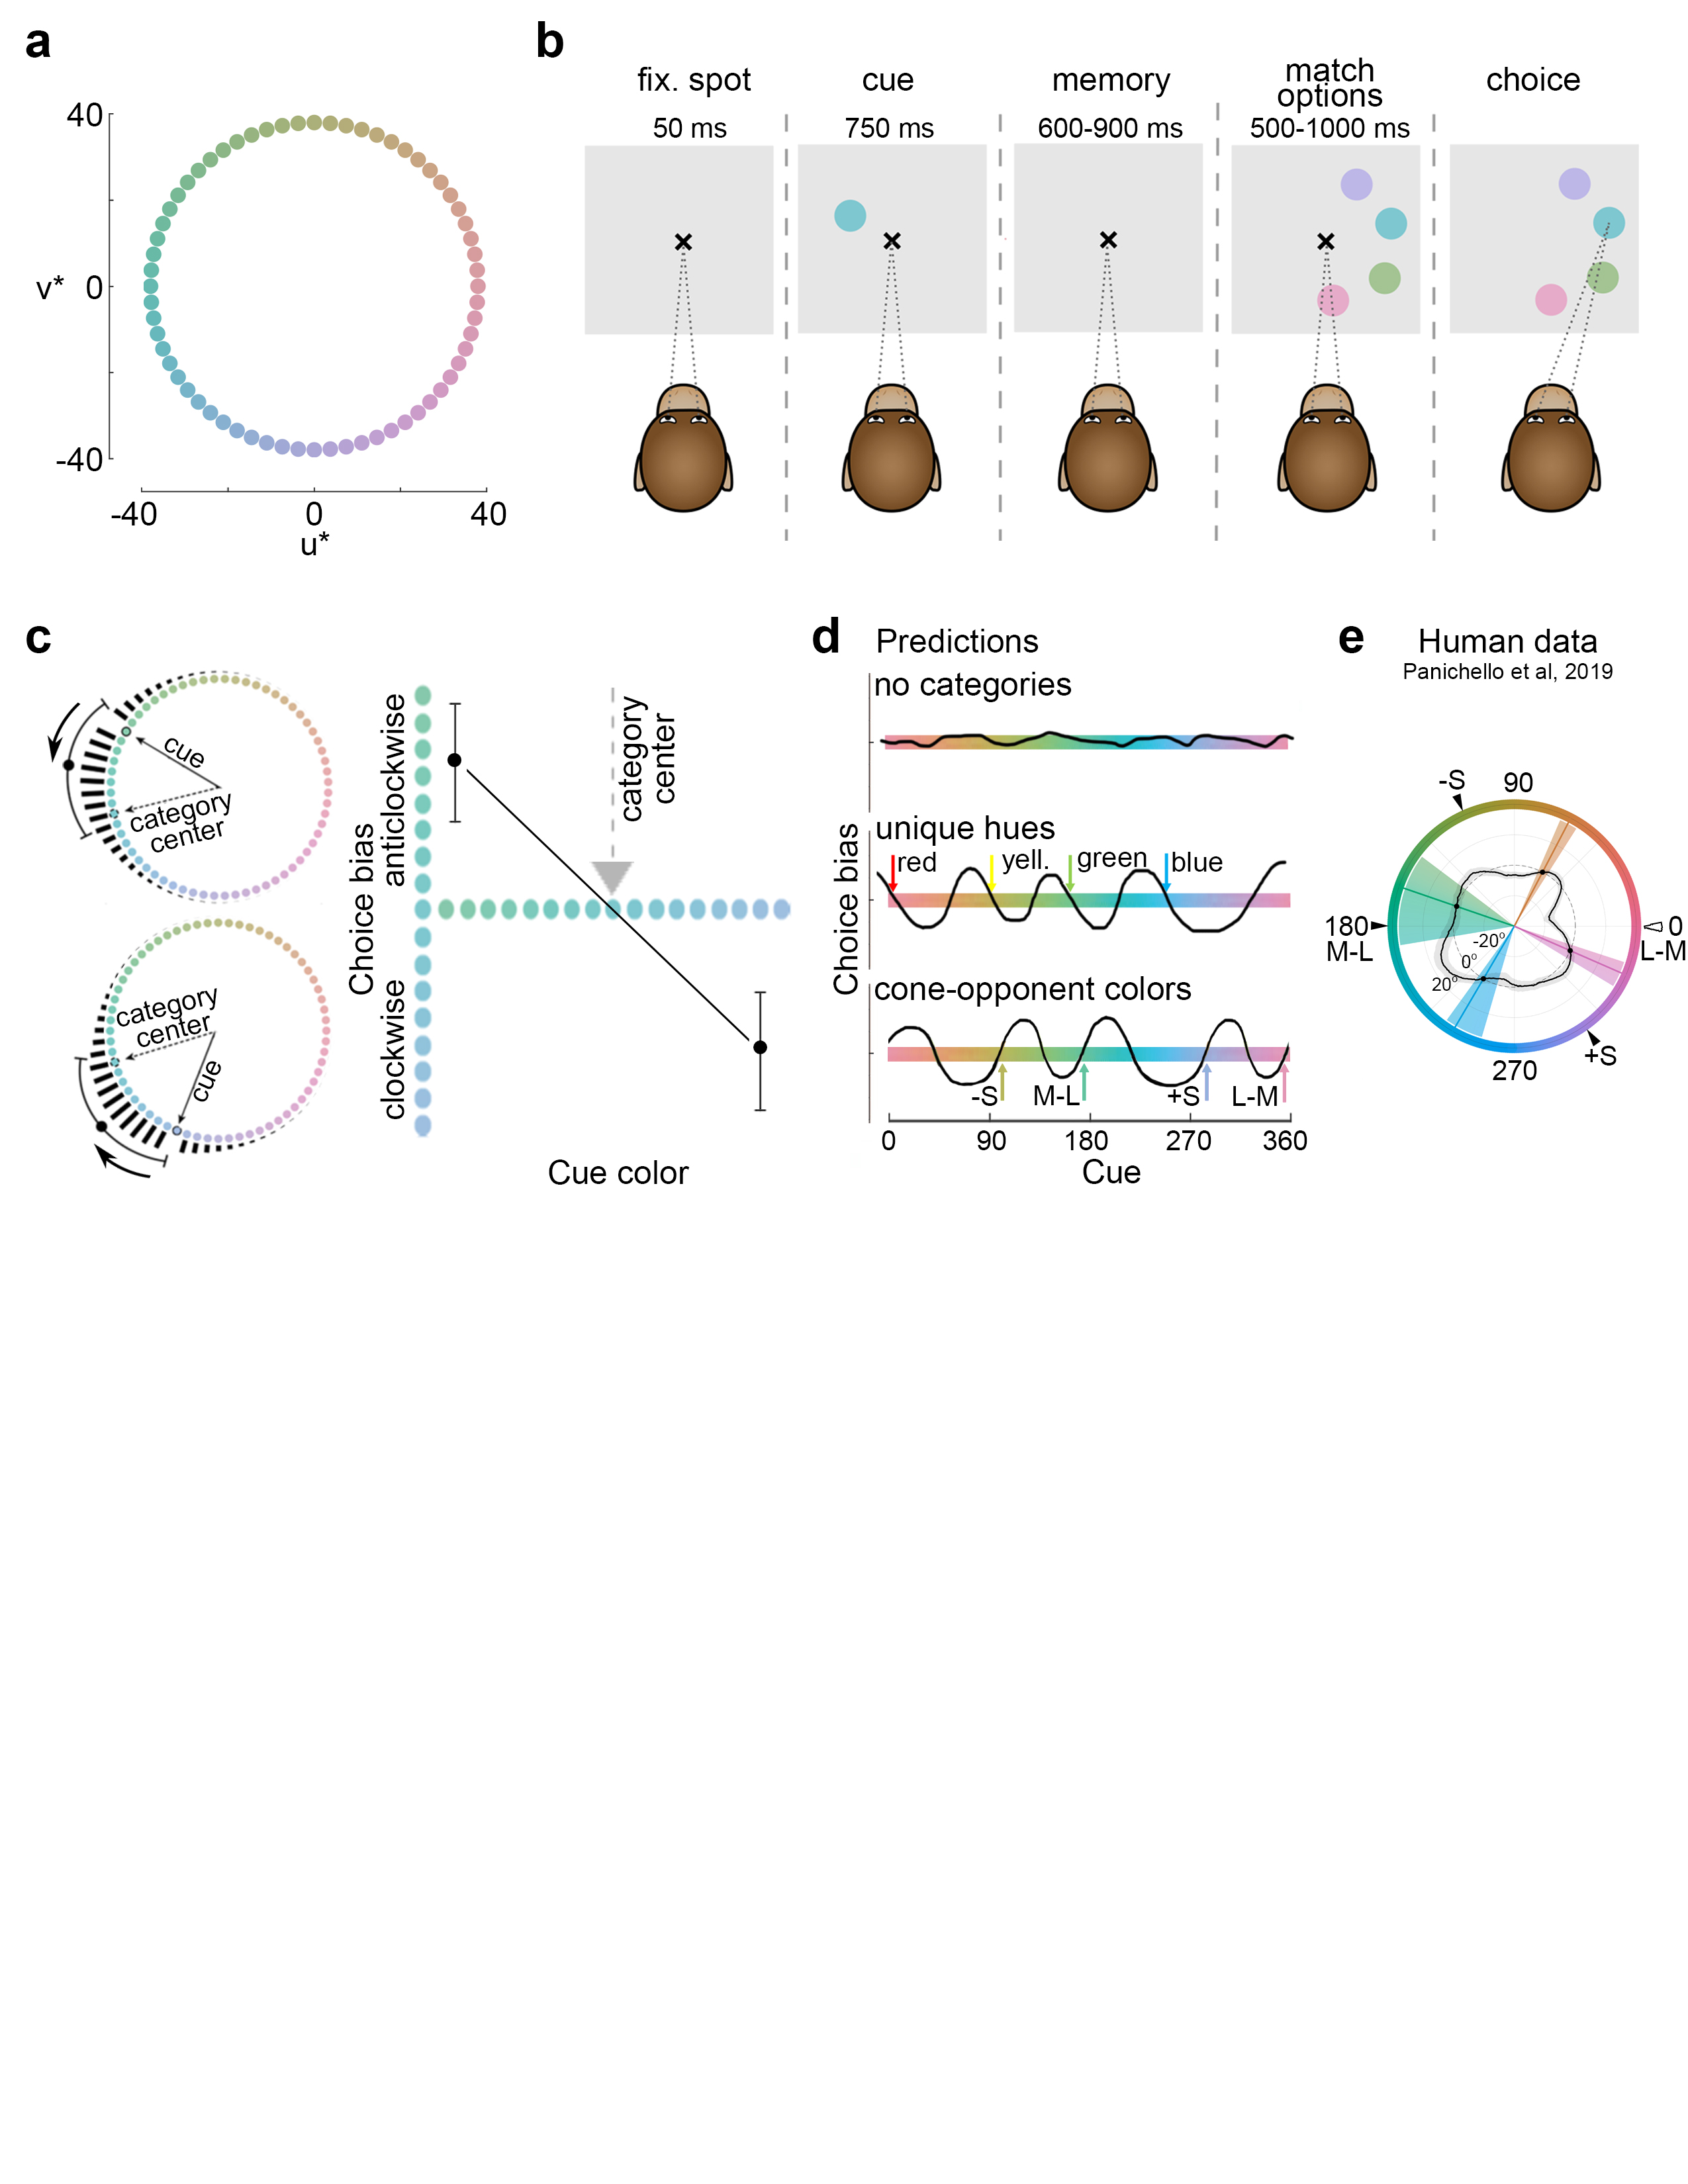
\includegraphics[width=\textwidth+4cm,trim={0 12.5cm 0 0},clip]{../Figures/flat/Fig1_ParadigmPredictions_7.jpg}
    \caption{\textbf{Non-verbal paradigm to recover color categories in non-human primates.}
    \textbf{a}, Sixty-four Colors defined in CIELUV color space. 
	\textbf{b}, Animals were trained to initiate a trial by fixating a small cross on a computer monitor and to maintain fixation throughout the trial until the fixation cross disappeared, which was their instruction to make a choice; trials in which the animals broke fixation were aborted. 
	A 3-degree diameter cue was presented within the central 2.5 – 6-degrees, followed by a variable memory delay (600-900ms) and the presentation of four choice options. 
	To mitigate impulsive choices, the choice options were shown for a variable amount of time (500-1000 ms) during which the animals needed to maintain fixation to avoid aborting the trial. After the fixation cross disappeared, the animals were free to make their selection. 
	\textbf{c}, Predicted distribution of choices for two cues if a color category exists at the specified location in the color space (dashed arrow). 
	The average of the distribution of choices will be shifted counterclockwise from the cue if the cue is displaced clockwise to the category center (top) and shifted clockwise from the cue if the cue is displaced counterclockwise to the category center (bottom). This pattern of results would be captured as the zero-crossing of the negative slope in a plot of the choice bias versus cue color (right). 
	\textbf{d}, Predicted pattern of results for three hypotheses: no categories (top); categories defined by attractors to the four common basic color categories (middle); and categories defined by repellors to the cone-opponent retinal encoding mechanisms (bottom). 
	\textbf{e}, Data obtained in prior work on a related task in human subjects showing evidence of four color categories (see SI Figure 2 for three other data sets in human subjects, showing a similar pattern of results). The negative slopes demarking category centers are recovered by tracing the line in a counterclockwise direction, at points where the trace crosses the dashed circle marking zero choice bias. For reference, arrowheads show the colors that would maximally activate the retinal cone-opponent encoding mechanisms (L-M, M-L, +S, -S; where L, M, S are the three cone types).}
    \label{fig:ParadigmAnalysisPredictions}
    \end{fullwidth}
\end{figure}

Color categories are identified by color terms, of which the Basic Color Terms are considered prominent \citep{berlin_basic_1969}.
One hypothesis is that a subset of these terms express, such as red, green, blue, and yellow, express universal concepts \citep{heider_universals_1972,regier_focal_2005}
and are endowed by hard-wired neural mechanisms present at birth \citep{bornstein_categories_1976,lindsey_universality_2006}. 
This idea, put forth 150 years ago \citep{hering_zur_1875}, predicts common patterns in color naming across cultures \citep{baronchelli_modeling_2010,lindsey_hunter-gatherer_2015,abbott_focal_2016}
and finds some neurophysiological support in human infants \citep{clifford_electrophysiological_2009,yang_cortical_2016}. 
Behavioral work in infants also provides evidence for a biological origin of color categories \citep{franklin_new_2004,ozturk_language_2013} and suggests that color categories may build on an innate scaffolding defined by retinal cone-opponent mechanisms \citep{skelton_biological_2017}.
The infants in all these experiments were at least several months old, by which stage they would have had substantial cultural exposure, so the evidence that they express color categories cannot be conclusively ascribed to an innate origin. Another hypothesis is that color categories emerge in development, instructed by language and culture starting at birth \citep{davidoff_colour_1999,roberson_color_2005}, possibly involving an interplay of innate and developmental factors \citep{webster_variations_2002,kay_language_2006,franklin_lateralization_2008,regier_language_2009,paramei_online_2018}---such an influence of cultural factors would explain the variability in color naming patterns across languages \citep{davidoff_colour_1999,webster_variations_2002,roberson_color_2005,kay_language_2006,gibson_color_2017, paramei_online_2018}. Current consensus is that at least some aspect of color category behavior is acquired through experience. But the extent to which color categories are innate remains unresolved \citep{davidoff_nature_2009,RN18696,RN18699}.

An alternative approach to studying the origin of color categories could be provided by behavioral experiments in trichromatic non-human primates \citep{RN18699,siuda-krzywicka_biological_2019}. 
The few studies on this topic have come to different conclusions: one found color categories in macaque monkeys consistent with categories in human adults \citep{sandell_color_1979}, implying that color categories do not depend on language and may be innate.
This study inadvertently made comparisons substantially easier for cross-category than within-category trials, undermining its conclusion \citep{davidoff_cross-species_2010}. 
A later study tested for the existence of color categories across a limited range of colors and found a blue-green boundary in humans but not baboons \citep{fagot_cross-species_2006,RN18699}. The lack of color categories in the baboons might reflect the limited survey of color space or the choice of colors (blues and greens are categorized with high variability in all languages, including English \citep{gibson_color_2017}). A third study, designed to investigate visual working memory, had two animals match color samples to a continuous ring of colors; it was inconclusive about consensus color categories in monkeys because the two animals showed a different pattern of results \citep{panichello_error-correcting_2019}.

\paragraph{Measuring color categories in macaque monkeys}

Addressing the question of color categories in monkeys requires overcoming several challenges. First, how can color categories be measured without teaching the animals the categories or reinforcing idiosyncratic biases \citep{essock_color_1977,matsuno_color_2004}? Second, how should the color stimuli be specified \citep{siuda-krzywicka_biological_2019}? For example, specifying the colors as wavelengths \citep{sandell_color_1979} is not appropriate \citep{davidoff_cross-species_2010}. 
Third, how can data across the full circle of hues be obtained so as to avoid missing categories \citep{fagot_cross-species_2006}? A match-to-sample paradigm, using colors defined in a perceptually uniform color space \citep{stockman_colorimetry_2010} (Figure 1a), provides a potential solution to these challenges, because, as demonstrated for human subjects , color categories introduce biases in the distribution of matches \citep{bae_why_2015}. So color categories could be inferred from any observed biases without resorting to language. 

In the standard paradigm, the subject is asked to match the color of a cue to a continuous ring of colors \citep{wilken_detection_2004,zhang_discrete_2008,bae_why_2015,panichello_error-correcting_2019,schurgin_psychophysical_2020}, which works in human participants who can follow instructions but introduces complications in monkeys because it is not clear how to reward the animals. Rewarding them for picking a color in the vicinity of the color of the cue could reinforce idiosyncratic biases\citep{panichello_error-correcting_2019}; moreover, the response metric (an eye movement or pointed finger) could confound the perceptual decision with motor noise. So we adapted the paradigm as an alternative-forced-choice task in which a direct match to the cue was available in every trial and the monkeys were only rewarded for making the direct match (Figure 1b). The precision of the eye tracker (\textasciitilde0.3 degrees of visual angle) was considerably finer than the size of the choice options (3 degree diameter). One consequence of the adapted paradigm is that it requires a large number of trials to sample category performance across the space of colors. Four animals performed the task, completing a total of 209456 trials over 232 sessions (SI Figure 1).

If a monkey has a color category, the category center will be an attractor in the color space. An attractor would be captured by a zero-crossing of negative slope in a plot of choice bias (Figure 1c). Repellors, meanwhile, would be captured by zero-crossings of positive slope. The approach is data-driven, so it will recover whatever categories exist; nonetheless, before collecting the data we considered three possibilities. First, that the monkeys would show no color categories, predicted by the work sampling a limited range of colors in baboons \citep{davidoff_cross-species_2010} (Figure 1d, top). Second, that the monkeys would show four color categories, predicted by attractor points defined by basic color terms (Figure 1d, middle). Third, that the monkeys would show four color categories, but predicted by data in human infants corresponding to repellor points defined by cone-opponent mechanisms not basic color terms \citep{skelton_biological_2017} (Figure 1d, bottom). For reference, Figure 1e shows the results in human adults \citep{panichello_error-correcting_2019}. These results have been replicated by several groups, across multiple versions of the task including the discrete-matching version used presently (SI Figure 2). Note that the data do not perfectly line up with color categories predicted by the four most common basic color terms (red, yellow, green, blue). Instead they correspond to pink, orange, green, blue. The discrepancy may arise because of limitations imposed by ensuring equal saturation and luminance among the colors (the resulting set of stimuli have neither a good red nor a good yellow) (see \citep{bae_why_2015}). 


%\section{Results}

\paragraph{Monkeys exhibit biases} %hallmarks of color category behavior

The animals examined show a hallmark of color categorization behavior: memory biases towards a set of particular points in a perceptually uniform colorspace.
In \autoref{fig:BiasCurves} it can be seen that the biases deviate substantially and systematically from zero, with the attractor points being found where the bias line crosses the zero line from positive to negative (going counter-clockwise). These points are highlighted with colored lines, with the filled areas around these lines showing the confidence intervals on these crossing points. Repeller points found where the line crosses the zero line from negative to positive.

\begin{figure}
\includesvg[width=\linewidth]{../../../Analyses/combined/combined_categorybias2_230214.svg}
\caption{\textbf{Bias as a function of hue, for data collapsed over 4 animals.} 
}
\label{fig:BiasCurves}
\end{figure}

\paragraph{Shared color categories across monkeys}

We see that all tested monkeys share two common attractor points, which we interpret as evidence of two shared color categories: a warm/orange-ish category (between 0$^\circ$ and 45$^\circ$), and a cool/blue-ish category (between 180$^\circ$ and 225$^\circ$).

\paragraph{Individual differences between monkeys}

In one animal we see evidence of additional categories: strong evidence for a greenish category and weak evidence for a purple category (the ``strength" of a category can be gleaned from looking at the local gradient at the zero-crossing point)

% Results table?

%\begin{figure}
%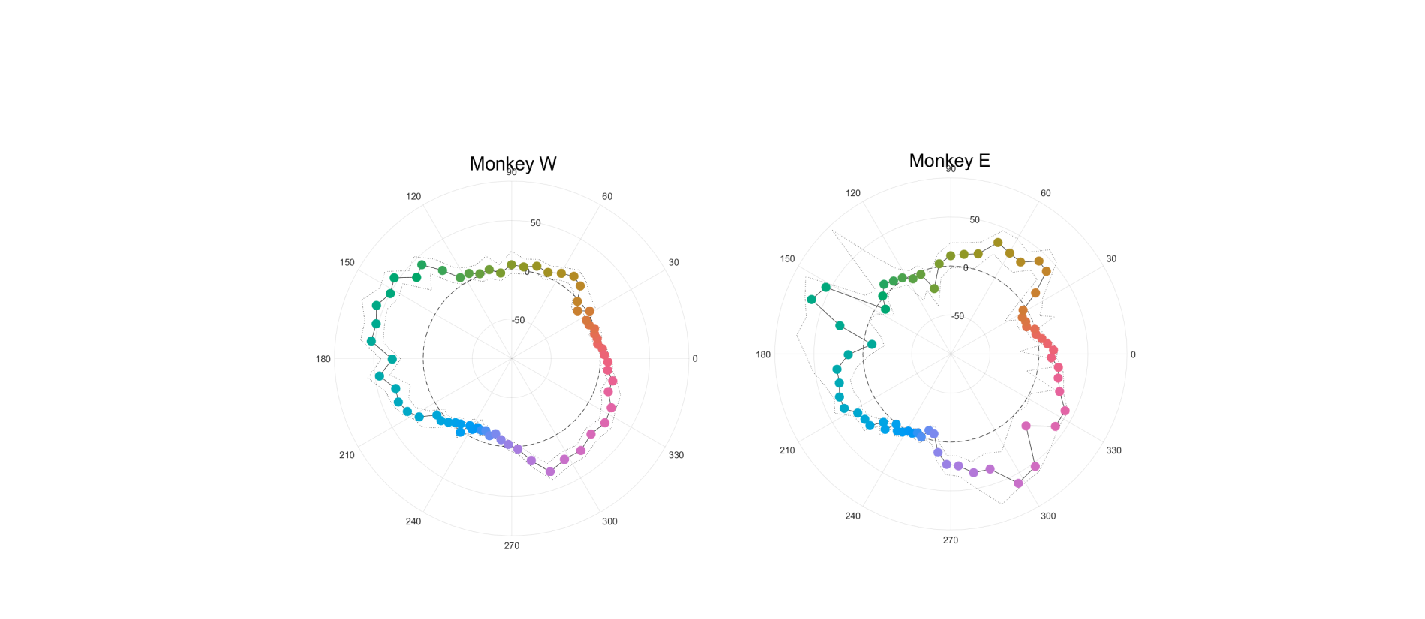
\includegraphics[width=\textwidth]{../../Figures/Old/panichellobias.pdf}
%\caption{Bias as a function of hue, for Panichello monkeys} 
%\end{figure}

\paragraph{Biases Compared to Humans}

Comparison to \cite{bae_why_2015}

Comparison to \cite{panichello_error-correcting_2019}

\paragraph{Cognitive Bias vs. Non-uniformity in Perceptual Space}

\begin{figure}
\includesvg[width=\linewidth]{../../../Analyses/combined/combined_TCC_230214.svg}
\caption{\textbf{Free Similarity model fit for combined data from all animals}
Similarity between stimulus $s_i$ and stimulus $s_j$, where one is the cue and one is the choice. This is a ``free'' similarity matrix - in that no particular relationship is pre-supposed between any of the stimuli (such as, for example: closer stimuli will be more similar). This figure can be compared to Figure 1D in \cite{schurgin_psychophysical_2020}, except there the rows are circularly shifted so that the the x-axis becomes the relative distance, rather than the absolute value of the stimulus. % should we just plot it the same way at this stage? It doesn't really make a difference here...
% supplementary figure with alternative plotting method?
%confidence intervals?!?!?! !!!!!!!!!!!!!!
} 
\label{fig:SimilarityMatrixCombined}
\end{figure}

\begin{figure}
    \centering
    \begin{subfigure}[b]{0.49\textwidth}
         \centering
         \caption{}
         \includesvg[width=\textwidth]{../../../Analyses/210609_124628_Buster/TCC_Buster_20230213.svg}
         \label{fig:SimilarityMatrixPollux}
    \end{subfigure}
    \hfill
    \begin{subfigure}[b]{0.49\textwidth}
         \centering
         \caption{}
         \includesvg[width=\textwidth]{../../../Analyses/210609_124628_Buster/TCC_Buster_20230213.svg}    
         \label{fig:SimilarityMatrixCastor}
    \end{subfigure}
    
    \begin{subfigure}[b]{0.49\textwidth}
         \centering
         \caption{}
         \includesvg[width=\textwidth]{../../../Analyses/210609_124628_Buster/TCC_Buster_20230213.svg}    
         \label{fig:SimilarityMatrixBuster}
     \end{subfigure}
     \hfill
     \begin{subfigure}[b]{0.49\textwidth}
         \centering
         \caption{}
         \includesvg[width=\textwidth]{../../../Analyses/220823_081207_Morty/TCC_Morty_20230213.svg}    
         \label{fig:SimilarityMatrixMorty}
     \end{subfigure}
        \caption{\textbf{Free Similarity model fits combined for individual animals} blabalbla}
        \label{fig:SimilarityMatrixIndividual}
\end{figure}


\paragraph{Longitudinal analysis}

Segmenting our data into subgroups of 5000 datapoints allowed us to both look at whether the determined categories varied over time, and also allowed us to perform a power analysis. From the monkeys studied it was clear that during our data collection period the categories remained static (within our measurement uncertainty), and also that the categories we saw are reliable enough to be seen with substantially less data. See Figures XXX % \autoref{}

% \section{Discussion}
% 
\paragraph{Locations of category centers.}

In the absence of language, we can infer that the shared categories we observe arise either due to innate biological factors, environmental factors such as the distribution of colors in the terrestrial environment, or a combination of the two.
The categories that we identify align well with the daylight locus (the line between the blue of the daytime sky, and the yellow of the sun, which itself closely follows the planckian locus), and also the warm/cool object/background distinction previously identified \citep{rosenthal_color_2018}. It is plausible that what we observe is the presence of two fundamental categories - `likely to be object of interest' and `likely to \emph{not} be object of interest'. 

\paragraph{Limitations of colorspace.}

For these experiments we used a nominally perceptually-uniform colorspace: CIELUV. This space has been derived psychophysically, with the goal of minimizing differences in perceptual non-uniformity across the space, for color differences of small magnitudes (the apparent color difference between two points in one part of the space should be equal to the apparent color difference between two points in another part of the space, given that the cartesian distance between the two points in each case be the same).

However, non-uniformities within the space are known to exist (ref?), and uniformity for small color differences does not necessarily assure uniformity for larger color differences (ref? Teunissen?). Likewise, uniformity for the conditions under which the psychometric measurements from which the space was determined (considering: spatial, temporal, spectral etc.) does not necessarily assure uniformity across all possible viewing conditions (ref).

With this in mind, it is reasonable to consider what the effect of residual non-uniformity might be on the results of our experiment. As discussed by \cite{panichello_error-correcting_2019} (their Figure S5) non-uniformities in colorspace could also potentially lead to systematic biases on tasks such as ours. The logic goes as follows: our points are uniformly distributed in our chosen space (\autoref{fig:StimuliAndParadigm}A), but if this space is actually non-uniform compared to the colorspace implicitly being used by an observer, then these same points will be \emph{non}-uniformly distributed in a hypothetical `perfect colorspace'. It follows that for each cue color, surrounding distractor points might actually be closer or further away than anticipated. If the nearest neighbors on one side of the cue are actually chromatically closer than the neighbors on the other side, one would expect these to be chosen at a higher frequency than the others, creating a systematic bias.

Unfortunately, these biases act in a similar fashion and are difficult to separate from one another. One potential way to distinguish one type of bias from another is to consider the theoretical relationship between bias and variance: if biases arise due to non-uniformities in colorspace, we would expect the attractor points to also have the \emph{highest} variance in responses. This is because in the hypothetical `perfect space' these points are actually tightly clustered, and so in the presence of noise we can assume that they will be frequently picked over one another. Conversely, at attractor points in spaces where the bias results from categoricality, theory would predict that we would see the \emph{lowest} levels of variance - if these points are conceptualized as `magnets' or `valleys' then we would expect cumulative noise to preferentially return to the attractor point, reducing the variance in responses.

In our data, we see...

[Compare to Bae/Panichello]

\begin{figure}
%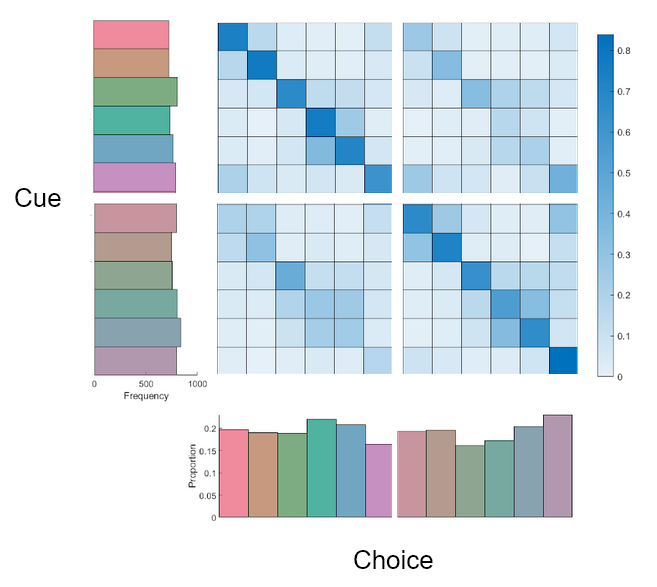
\includegraphics[width=\textwidth]{../../Figures/saturationBias.png}
\includesvg[inkscapelatex=false, height=\textwidth]{../../Figures/working/Poster_components/SD_Pollux copy.svg}
\caption{\textbf{}}
\label{fig:SamplingBias}
\end{figure}
\paragraph{Saturation bias.}

Non-uniformities in CILUV may also plausibly result in our nominally iso-saturated colors actually being variably saturated. This would be a concern, as it would be a reasonable prediction that higher saturation colors would be more salient, and thus more likely to be selected as responses. In a control experiment we see no (or very little) bias towards higher saturation colors. In \autoref{fig:saturationBias} it can be seen that there are a reasonable number of errors where an animal picks a higher saturation version of the same hue (lower left quadrant), but it is also seen that the number of errors of the inverse type (upper right quadrant) are roughly equal in number.


\begin{figure}
%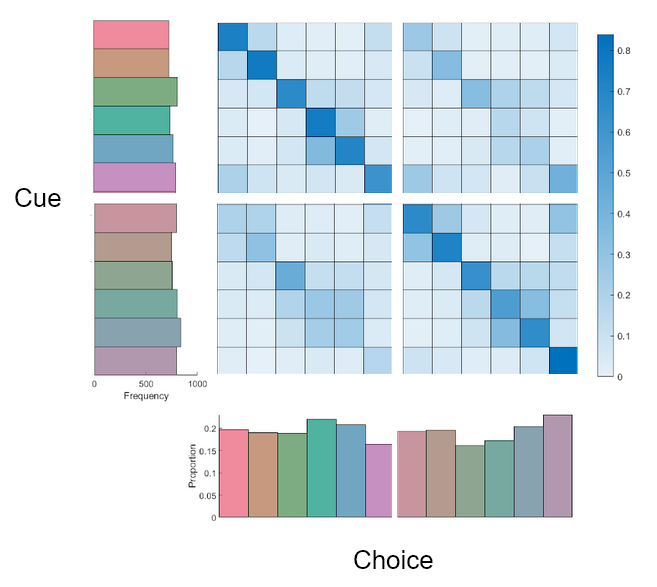
\includegraphics[width=\textwidth]{../../Figures/saturationBias.png}
\includesvg[inkscapelatex=false, width=\textwidth]{../../Figures/working/Poster_components/Saturation copy.svg}
\caption{\textbf{Saturation Bias.}
Heatmap of cues and corresponding choices. Selections along the negative diagonal correspond to correct choices. Choices along the negative diagonal in the bottom left and top right quadrants show trials on which an incorrect choice was made in such a way that the hue was correct but the higher or lower saturation versions of the cue were chosen (respectively). Note: the main diagonal is expected to be filled in at a greater extent regardless of performance level, since the correct choice is shown on every trial, whereas only a subset of the incorrect choices are shown.}
\label{fig:saturationBias}
\end{figure}



\paragraph{Comparison with humans} % /Panichello

%\section{Conclusion}

\printbibliography[title=Main Text References]
\end{refsection}

% DON'T EDIT. If "endfloat" option is enabled all floats appear before appendices
\if@endfloat\clearpage\processdelayedfloats\clearpage\fi 

\begin{refsection}
\newpage

\section{Methods}
\subsection{Subjects}

Data were collected in four adult male rhesus macaques (Macaca mulatta)(“PO, CA, BU, and MO”) weighing 8–10 kg. 
All experimental procedures were approved by the Animal Care and Use Committee of the National Eye Institute and complied with the regulations of the National Institutes of Health. 
Plastic headposts were mounted with sterile surgical procedures, using procedures described in detail elsewhere \citep{lafer-sousa_parallel_2013}. 
The animals were acclimatized with positive reinforcement to sit in a custom-made chair positioned with the eyes 70cm in front of a computer monitor and to perform visual tasks as described below. 
At the beginning of each testing session, we positioned a mouthpiece to deliver fluid reward to the animal. 
An infra-red camera was directed at the eye to monitor eye position with the ISCAN system. 
The precision of the eye tracking was \textasciitilde0.3 degrees. 

\subsection{Behavioral task}

The animals were trained to perform a 4-Alternative Forced Choice (4-AFC), Delayed Match to Sample task, in which they were shown a colored cue and rewarded for selecting the match option that had the identical color (see Figure 1). 
The colors, described in more detail below, were drawn from a set of 64 colors that evenly sample hue angle of CIELUV color space \citep{stockman_colorimetry_2010}. 
Each trial was initiated when the animal fixated a small cross at the center of the screen; trials were aborted if the animal did not maintain fixation until the fixation cross disappeared toward the end of the trial. 
Fixation was defined as within a 1.5 degree wide area centered on the fixation cross, well within the precision of the eye tracker.
The trial sequence was as follows. 
Fifty ms after initiating the trial by fixating the central cross, a 3-degree-diameter “cue”  of a color randomly drawn from the set of 64 colors appeared for 750ms. 
The cue was positioned on the monitor at the same location for all trials during a given daily recording session.
From day to day, the position of the cue could vary, from 2.5-degrees to 6-degrees eccentricity (measured at the center of the cue) and be at any angle from fixation.
The cue was followed by a gray screen for a brief “memory” period of 600-900ms, after which four match options appeared along an arc at an eccentricity of 6-degrees. 

One match option was always a direct match to the cue, and the other three were randomly sampled without replacement from the remaining 63 stimuli. The match options had the same shape and size as the cue (3-degree-diameter discs); they were evenly spaced along the arc, with a gap of 2 degrees separating each option. In all animals except one (CA), the arc along which the match options were placed was in the visual hemifield opposite to the cue. The exact position of the arc within the hemifield varied from trial to trial, so the animals could not anticipate where the choice options would appear. Animal CA had a small scotoma spanning \textasciitilde3degrees of visual angle in a quarter of the visual field as the result of a \textasciitilde3mm diameter V1 lesion, so the cue and choices were placed in the same (intact) hemifield, taking care to avoid overlap of the position of the cue and the choices. 

After a random period from 500-1000 ms, the fixation cross disappeared, instructing the monkey to direct its eyes to one of the choices. This random period helped guard against the animals making impulsive responses because they could not anticipate when exactly the choice options would appear. Reward was given only if the animal selected with an eye movement the choice that was identical to the cue. 
If the monkey failed to make a choice within 5 seconds or broke fixation at any point before the termination of the fixation cross, the trial was aborted.

The experiment was controlled with custom software written in MATLAB and Psychtoolbox \citep{noauthor_nei-lsrkofiko_2022, kleiner_whats_2007}.

\paragraph{Stimuli}
Stimuli were 3-degree diameter discs presented on a Cambridge Research Systems Display++ screen. 
Colors were defined to be on an equiluminant plane in CIELUV color space, with the luminance matched to the adapting gray background (L* = 76.0693, 38.5cm/m2; adapting field chromaticity was xy\textsubscript{1931}: 0.2684, 0.2409). 
The stimulus set included 64 colors, evenly sampling CIELUV hue angle (5.625-degrees between adjacent stimuli), of equal CIELUV saturation (radius 37), the highest saturation possible for a set of stimuli of equal saturation and luminance given the gamut of the display.
Luminance contrast noise was randomly added to each pixel of the cue and the match options to mitigate chromatic aberration. 
The luminance added to each pixel was updated every frame and drawn uniformly from a continuous range of +/- 5 L* units (the resulting stimulus looks like a colored disc viewed behind a thin veil of television snow). 
CIELUV was used to define the stimuli because it has an associated chromaticity diagram, but the stimuli can readily be transformed into other spaces such as CIELAB and DKL. 

The color stimuli corresponding to the poles of the cone opponent cardinal axes, labeled in the polar mixture model plots, were computed as follows. 
CIELAB and CIELUV values were transformed to XYZ coordinates using the PsychToolbox functions “LabToXYZ” and “LuvToXYZ” respectively.
An XYZToLMS matrix was constructed using MATLAB's “mldivide” function with the Smith-Pokorny cone fundamentals and the CIE XYZ standard observer color matching functions as inputs.
The PsychToolbox function “ComputeDKL\_M” was then used to compute a conversion matrix for converting between LMS and cone opponent cardinal axes that define the DKL colorspace. 
The code which accomplishes the above is available \href{https://github.com/NEI-LSR/MacaqueColorCategories/blob/main/Analyses/DKL/computeDKL_XYZ.m}{here}.

\paragraph{Human Data}

Data from published reports using two related tasks completed in human subjects were kindly provided by Gi-Yeul Bae \citep{bae_why_2015} and Timothy Buschman \citep{panichello_error-correcting_2019}.
Both these data sets involved a paradigm in which participants matched the color of a cue to a ring of colors showing a continuous progression of colors around the color circle (a ``color wheel''). 
The results of the two prior studies are consistent with each other: when analyzed with a mixture model, both data sets show four color categories corresponding to blue, green, orange, and pink (SI Figure 1); moreover, the results on a version of the task that omits the memory delay period also recover these four color categories \citep{bae_why_2015}.
This prior work shows that the results on the color-matching task are reproducible and robust. 
It is therefore likely that the results of the present version of the task, which is distinguished from the prior work by providing as options discrete targets as opposed to a continuous colored wheel, would also be similar. 
But to test this likelihood, we recruited human participants via Amazon Mechanical Turk to perform the same task used in the macaque monkeys in the present work. 
To request a trial, participants used a mouse to adjust the location of a cursor to click on a fixation cross, after which a cue was shown to one side of the fixation cross, and the cursor disappeared. The cue was displayed for 750 ms. 
After the cue was extinguished, a fixation cross was shown but the cursor remained hidden to de-incentivize mouse movement (1500 ms). Four choices were then shown, and the cursor reappeared; participants made their selection by using the mouse to move the cursor to their choice and clicking the mouse. 
All other aspects of the experimental design were the same as the experiment deployed with the monkeys: 64 colors of equal saturation and luminance (we assumed the monitor that each on-line participant was using matched the sRGB standard), evenly sampling CIELUV. 
The pattern of results was consistent with the published studies using the continuous ring of colors, recovering four significant color categories corresponding to blue, green, orange, and pink (SI Figure 1; see Data Analysis: Mixture Modeling for a description of how these data were analyzed). %!!!!!!

\subsection{Data Analysis}

\paragraph{Psychometric functions}

Psychometric functions (see Figure 2a, SI Figure 2) were estimated with a Weibull cumulative density function: %!!!!

\begin{equation} \label{eq:Weibull}
    y=\zeta+(100-\zeta-\gamma) *\left(1-e^{-(\omega / \lambda)^k}\right) 
\end{equation}

Where animal performance (y) is a function of trial difficulty ($\omega$), computed for each trial as the angular difference between the color of the cue and the color of the foil with the closest color to the cue. 
The other parameters are the floor of the function ($\zeta$), the ceiling ($\gamma$), slope ($\lambda$), and inflection point ($k$). 
All completed trials were included in the analysis of the psychometric functions. 
The number of completed trials for each animal were: 76121 (PO); 54555 (CA); 24526 (BU); 54252 (MO). 

\paragraph{Mixture Modeling}\label{para:MixtureModeling}

Following experiments in human subjects, we analyzed the distribution of color matches made to each color using a mixture model \citep{zhang_discrete_2008,bae_why_2015}; this model assumes that the shape of the distribution is normal and provides an estimate of the width of the distribution, the offset (or bias) of its peak relative to the target color, and the guess rate.
Prior work has done this analysis with a von Mises distribution \citep{zhang_discrete_2008,bae_why_2015}.
We found it simpler to implement it with a Gaussian function, $f(\theta)$:

% demo annotated-equation code from here: https://mirrors.concertpass.com/tex-archive/macros/latex/contrib/annotate-equations/annotate-equations.pdf

%\newpage %Sometimes the annotations don't show up, the hacky solution is to force them onto a new page

\begin{equation} \label{eq:GaussianEquation}
    f(\theta) = {\alpha} \cdot e^{-\frac{(\theta-{\mu})^2}{2{\sigma}^2}} + {\zeta}        
\end{equation}

% \vspace{2em} 
% \begin{equation} \label{eq:GaussianEquation}
%     f(\theta) = 
%     \eqnmarkbox[purple]{alpha}{\alpha}
%     \cdot
%     e^{
%     -\frac{(x-
%     \eqnmarkbox[violet]{mu}{\mu}
%     )^2}{2 
%     \eqnmarkbox[blue]{sigma}{\sigma}^2}}
%     +
%     \eqnmarkbox[gray]{zeta}{\zeta}        
% \end{equation}

%\annotate[yshift=1em]{above,left}{alpha}{height of the curve's peak}
%\annotate[yshift=1em]{above}{mu}{position of the center of the peak}
%\annotate[yshift=-0.75em]{below,left}{sigma}{standard deviation}
%\annotate[yshift=-1em]{below}{zeta}{floor}
%\vspace{2em} 

where $\alpha$ is the height of the curve's peak, $\theta$ is the hue angle, $\sigma$ is the standard deviation (width), $\mu$ is the center of the peak (so the offset is $\theta$-$\mu$), and $\zeta$ is the floor (guess rate). 
To do the analysis, we used the MATLAB fit function, which was provided with the number of times each choice color was an option for the given cue across all completed trials and produced the best-fitting function along with the 95\% CI values for those parameters (SI Figure 3; note that the tails of the distributions in SI Figure 3 reach an asymptotic floor, justifying the use of the simpler Gaussian fitting procedure). 
The offset values for each cue were smoothed with a moving average spanning three colors (16.875 degrees) (Figure 2b and 2c, Figure 5a, and SI Figure 4). Negative-slope zero-crossings in which the 95\% CI exceeded the zero crossing were considered category centers (see Figure 1).

The width of distribution of matches varied among the colors; this was also observed by \citet{bae_why_2015} (see their Figure 7). 
This variation implies that the assumption of uniformity of the colorspace is not valid. 
Moreover, such a non-uniformity could yield an offset in the mixture model (see Figure 3), so any offsets recovered by the mixture model need not require a cognitive origin.  
The alternative hypotheses for the origin of offsets recovered by the mixture model (a cognitive origin versus a stimulus-space non-uniformity), prompted us to analyze the data with a more sensitive model, the Target Confusability Competition model \citep{schurgin_psychophysical_2020}.
We recognize that in principle, the mixture model could distinguish these alternative hypotheses, but we encountered some limitations using the mixture model that were readily overcome by the TCC model. 

\paragraph{Modified Target Confusability Competition Model (TCC-v)}\label{para:TCC}

The key elements of the TCC model are a similarity function, which determines the similarity between stimulus $s_i$ and stimulus $s_j$ through a non-linear mapping of distance in colorspace to perceptual similarity, and a value of $d'$, which can be thought of as describing the amount of noise acting in the system. 
These two elements can be used to predict the probability that a choice of colour $s_j$ will be picked from the set of $\left[s_{j1}...s_{jn}\right]$, on a trial where the cue is $s_i$. 

The probability of a particular choice being selected on a particular trial ($p_t(\text{selecting choice}_n)$) is dependent on the cue, the set of choices, the similarity function ($f(\theta)$), the value of $d'$, and the perceptual distances between stimuli ($D$).

\begin{equation} \label{eq:pt}
    p_t\left(\text{selecting choice}_n \mid \text{cue},\text{choices}_{i:j}, f(\theta), \delta, D\right)
\end{equation}

where $f(\theta)$ is the Gaussian equation (\autoref{eq:GaussianEquation}), $\delta$ is the value of $d'$, and $D$ is the perceptual distances between stimuli.

The TCC model has been deployed with the assumption that the colorspace is perceptually uniform \citet{schurgin_psychophysical_2020}; this assumption is implemented as a single similarity function fit for all stimuli. 
But, as \citet{schurgin_psychophysical_2020} demonstrate the similarity function need not be fixed (see their Figures 1d and Extended Data Figure 5). 
Our implementation of the model, which we call TCC-v, permits the similarity function to vary for each cue (the "v" is for vary). 

We created four versions of the TCC-v model: the "null model" (with only parameters for the Gaussian width of the similarity function and $d'$, and thus no allowance for bias), the "cognitive bias" model (with 64 parameters corresponding to offset values shifting the peak of the similarity function for each stimulus to higher or lower hue angles, in addition to $d'$ and gaussian width), and the "stimulus-space non-uniformity model" (with 64 parameters corresponding to the relative distance between each pair of neighboring stimuli, in addition to $d'$ and gaussian width). 
Finally, the "free-similarity" model, does not pre-suppose any specific similarity function; every cell in the similarity matrix is an independent parameter. 
This flexibility allows for patterns of similarity that are not captured by our hypotheses. 

In fitting the model parameters, our goal is to minimize the negative log likelihood (NLL) of the observed data. 
The NLL is computed as the sum of the negated log of the probabilities of the choices that were selected being selected. 

\begin{equation}
    \text{NLL} = \operatorname{sum}\left(-\left(\log \left(p_t\left(\text {selecting choice}_x\right)\right)\right)\right)
\end{equation}

where $\text{choice}_x$ was the choice that was selected on each trial.

The parameter estimates for the free parameters used by the model are iteratively updated until the model reaches a stable minimum NLL. 

The "null model" is defined by $f(\theta)$ (where $\alpha$ = 1, $\zeta$ = 0, $\mu$ = 0) and $d'$, and assumes $D$ to be uniform. 
The "cognitive bias" model is defined by $f(\theta)$ (with 64 parameters for $\mu$, 1 parameter for $\sigma$, $alpha$ = 1, $\zeta$ = 0) and $d'$, and also assumes $D$ to be uniform. 
The "stimulus-space non-uniformity" model is defined by $f(\theta)$ (where $\alpha$ = 1, $\zeta$ = 0, $\mu$ = 0) but specifies for each pair of neighboring stimuli a unique value for $D$ (64 parameters). 
Note that the cognitive bias model and the stimulus-space non-uniformity have the same total number of parameters (66). 
The "free similarity model" is not defined by $f(\theta)$; it is defined by $d'$ and the similarity matrix. 
The similarity matrix is defined by 4096 ($64^2$) parameters, one for each combination of cue and possible choice (note that the free similarity matrix is not required to be symmetric).

$p_t(\text{selecting choice}_n)$ is the probability that a sample drawn from an independent normal distribution $(X_i \sim N)$ is the highest of such samples drawn for all the choices ($i:j$) on a particular trial. 
The mean ($m$) of each distribution is defined by the similarity value for that cue/choice combination, multiplied by $d'$, and has a variance of 1.

\begin{equation}
    p\left(\text{selecting choice}_n\right) = 
    p\left(X_i \sim \mathcal{N}\left(m_n \cdot \delta, 1\right)
    >\max 
    \left(X_{i+1: n} \sim \mathcal{N}\left(m_n \cdot \delta, 1\right)\right)\right)
\end{equation}

where $m_{i:j} = f\left(|\text{cue}_{i} - \text{choices}_{i:j}|\right)$, and $\delta$ is the value of $d'$.

We used an AFC paradigm as opposed to a continuous response space, so we can take advantage of an alternative computational method for estimating $p_t(\text{selecting choice}_n)$, using correction factors provided by \citet{mcgraw_common_1992} (their Table 3). 
This decreases the amount of time taken to fit the TCC-v models. 
The method for computing $p_t(\text{selecting choice}_n)$ in the original TCC model of Schurgin et al. is provided here: \verb|modelPDF| in \verb|TCC_Code_InManuscriptOrder |\verb|\Model| \verb|\TCCUncorrelated.m| from \url{https://osf.io/j2h65/}. 
The method we used is provided here: \url{https://github.com/NEI-LSR/TCC_AFC}.

When fitting the free similarity matrix model, we fix $d'$ to provide a constraint on the floor and ceiling of values in the similarity matrix.
$d'$ is strongly correlated with the range of the values in the similarity matrix; the range of similarity values in the similarity matrix has a maximum span of 0 to 1. 
Equivalent NLL values can be obtained either by restricting the range (e.g. 0.49 to 0.51) and a high value of $d'$ (e.g. 20), or by having a larger range (e.g. the full 0 to 1) and a low value of $d'$ (e.g. 0.1). 
If $d'$ is not fixed, the model is as likely to assume a restricted range as it is a larger range (though still bounded between 0 and 1) but will take a long time to converge. 
Fixing $d'$ impacts the specific values (akin to increasing or decreasing the contrast of the similarity matrix image) but it does not impact the interpretation of the similarity matrix. 
We chose a $d'$ value of 1 which is a reasonable estimate for our task \citep{schurgin_psychophysical_2020}.

In the original TCC model, the similarity function uses two parameters that define a Gaussian function representing perceptual noise and an exponential function; these two functions are convolved (see Figure 1f of \citep{schurgin_psychophysical_2020}). 
We simplify the similarity function such that it is defined by a Gaussian alone. 
The cost of this is that it does not allow for a distinction between the impact of perceptual noise (where the curve flattens off approaching perceptual distances of 0) and similarity (the general shape of the function). 
In practice, we found that these parameters were highly correlated, and that reduction to a single parameter substantially reduced the computational cost of model fitting, and produced parameter estimates that were more resistant to variation in model-fitting starting values. 
This simplification also made it easier to modify the model; for example, to allow for the peak of the function to not be at 0 (this affords the TCC-v model the same ability as the mixture model to capture offsets).

\paragraph{Choice Probability Matrices vs. Similarity Matrices}

\begin{figure}
    \begin{fullwidth}
    \centering
      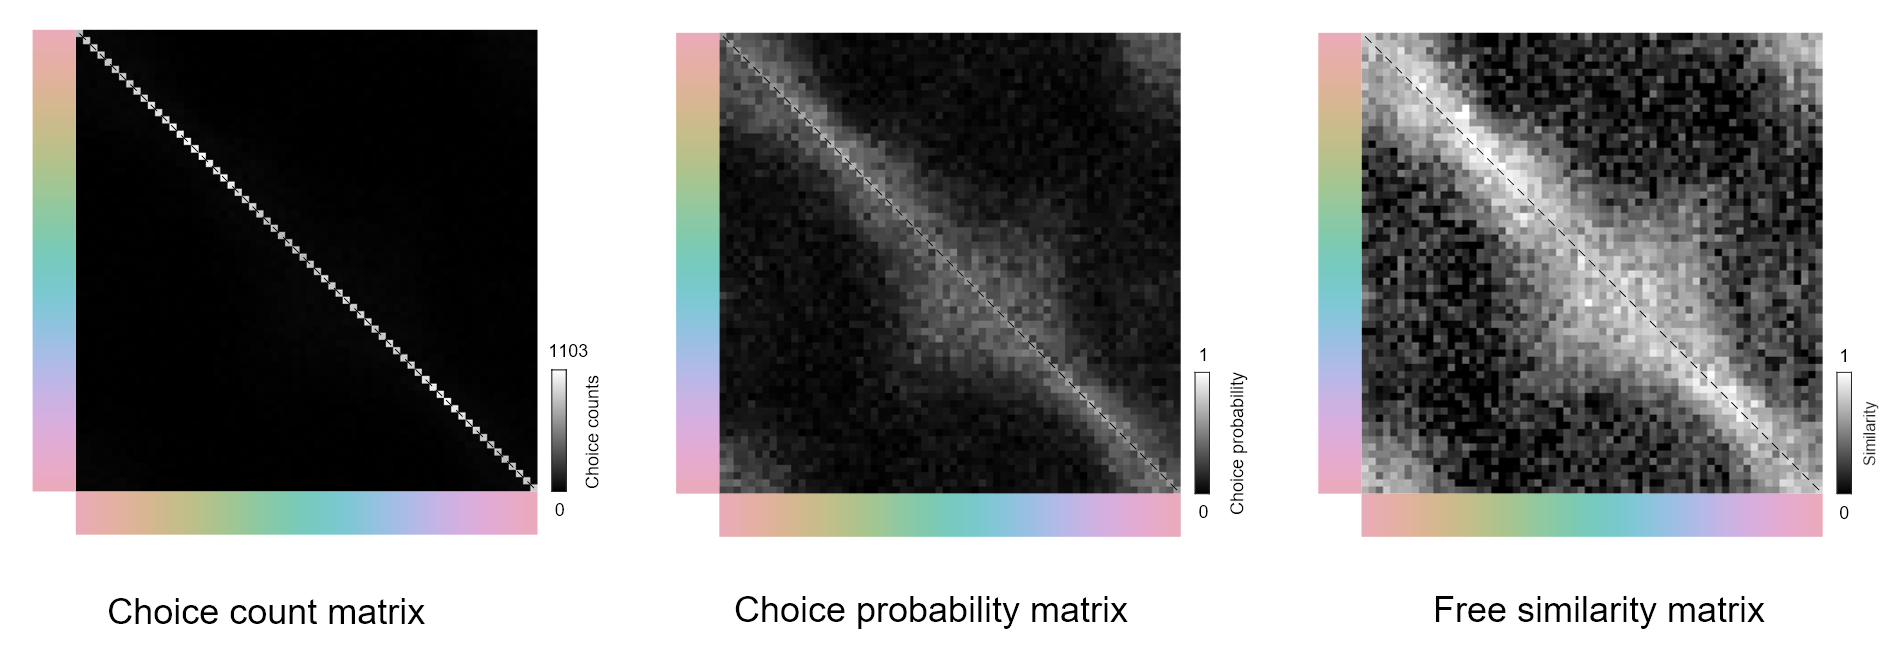
\includegraphics[width=\textwidth,]{../Figures/flat/F7_choiceProbVsSim.png}
           \caption{\textbf{Comparison of Choice Count Matrices, Choice Probability Matrices, and Similarity Matrices}.
           Choice count matrices describe the number of times a specific choice is made. 
           Choice probability matrices normalise for the number of times a particular choice was available as a choice option. 
           Similarity matrices are created through model fitting and represent the perceptual similarity between stimuli, and are beneficial since they are not influenced by mixed viability of distractors (see text for further details).}
		\label{fig:MACBEHcolorspace}
    \end{fullwidth}
\end{figure}

A choice probability matrix is a graphical representation of the probability that choice y will be chosen given cue x.
To construct such a matrix, one counts the choices which were made in response to each cue, producing what we can refer to as a choice count matrix, and then divides each cell by the number of times that each cue/choice combination was presented. 
This normalizes for the possibility that some cue/choice combinations were presented more than other combinations. 
This process disregards any information about what the unchosen distractors were on a given trial.

In paradigms which use a continuous response space the set of choices is the same on each trial – the full set of possible choices. 
This is not the case for our reduced AFC paradigm, and this introduces a potential issue which needs consideration.

Imagine a trial with three distractors which are all close to one another (let's say that they are 5, 6, and 7 colorimetric units away from the cue).
On another trial, imagine that one distractor is a much more viable choice option than the other two (let's say the choices are 5, 25 and 26 units away from the cue).
The odds of picking the distractor that is 5 units away is different on these two trials - it is more likely on the second trial, because the other distractors are less viable options. 
This becomes a potential issue because to counterbalance trials such that each cue is shown with the full set of possible distractors would require roughly 2.5 million trials (nchoosek(63,3) * 64).
Without counterbalancing, it is not possible to disentangle differences in choice probability which arise due to perceptual similarity (which is what we are aiming to measure) vs differences in distractor viability.

We avoid having to collect a complete set of 2.5 million trials by employing the concept of a similarity matrix.
A similarity matrix is the core component of a TCC-v model, and maps the similarity between cues and choices. 
Using it, the similarity between the cue and each of the choices on a particular trial (and also the similarity between each of the choices themselves) can be used to compute the probability of each choice being selected.
While we can compute the choice probability matrix rather simply, as described above, the creation of a similarity matrix requires a model-fitting approach – a similarity matrix is randomly initialized with values, and the likelihood of the data given that matrix is computed, then the matrix is randomly perturbed and the likelihood of the data is recomputed, and then perturbed again in whatever directions seem to increase the likelihood of the data, setting forth an iterative process whereby the similarity matrix is perturbed until a maximum in likelihood is reached, and our best estimate of the underlying similarity matrix is thus settled upon.
This is a computationally intensive process, and for datasets with many choices (such as those with a continuous response space), we have been unable to fit similarity matrices. 
Thankfully, there is a trade-off: data collected with continuous response spaces see less benefit of a similarity matrix over a probability matrix. 
For such datasets, as the number of trials increases the probability matrix increasingly approximates the similarity matrix.
It is expected that choice probability matrices and similarity matrices will be highly correlated and show the same structure.

A related issue, also addressed by employing the concept a similarity matrix, is the artifact caused by the inclusion of a direct match on every trial in our paradigm. 
This can be thought of as an unequal counterbalancing which no number of repeated trials would be able to balance out, but it is necessary for our training of the monkeys (since there needs to be a clear rubric for what choices are “correct” and thus rewarded).
Note how the choice count matrices and choice probability matrices for our data appear to show an elevated diagonal. 
The reason this exists in the choice count matrix is clear – those option are simply presented more frequently, but the reason this survives the normalization (by the number of times that each cue/choice combination was presented) is less obvious: any non-match choice which is close to the direct match will always have a viable competitor (the match), whereas the match choice won't always have a viable competitor (since it is possible that the distractors are all distant on a particular trial).
This leads to an increased probability of selecting the matching choice relative to an incorrect choice. This issue only affects choice probability matrices; it does not affect similarity matrices.

\paragraph{Quantitative Model Comparison}
To compare the relative performance of models, we computed Bayesian Information Criterion (BIC) values for each model from the NLL. 
The BIC values provide a unit by which we can assess whether the differences between NLL are meaningful, penalizing for number of parameters and number of trials. 
BIC also allows us to compare models with differing numbers of parameters (though note that the "cognitive bias" and "stimulus-space non-uniformity" models have the same number of parameters).

\begin{equation}
    \text{BIC} = k\ln(n)-2\ln(\hat{L})
\end{equation}

Where $\hat{L}$ is the maximised likelihood of the model, $n$ is the number of trials, and $k$ is the number of parameters.

To compare the relative performance of the cognitive bias and stimulus-space non-uniformity models we performed 100 bootstrap iterations of the analysis. 
Each bootstrap drew 24526 trials from the total number of completed trials for each animal (24526 was the minimum number of trials of completed trials among the 4 animals). 
Both models were then fit to each bootstrap iteration, and the BIC values were computed (see Figure 4d).

\paragraph{Reverse-engineering a uniform color space from the macaque color-matching data}

The present results imply that CIELUV is perceptually non-uniform; that is, that it samples with variable density the true underlying perceptual colorspace. 
The parameters of the stimulus-space non-uniformity model describe the relative positions of the stimuli, as determined empirically. 
After converting from inter-neighbor relative distances to polar angles, these can be thought of as the hue angles for the stimuli that we used, represented now in a behaviorally derived color space which we refer to as the Macaque Uniform Color Space (MUCS) (Figure 6b). 
The inverse transformation is also possible; we can define a set of hue angles that are uniformly distributed in MUCS and convert them into CIELUV. 
For example, if we define hue angle $i$ in MUCS, we can reparameterize that hue angle such that it is defined by its angle relative to the two experimental stimuli on either side of it (hue angle $i$ is at y\% of the angular distance on the path between experimental stimuli $a$ and $b$). 
We can then plot MUCS hue angle $i$ in CIELUV by plotting it at the location which is y\% along the path between experimental stimuli $a$ and $b$ in CIELUV. 
Such a set of hue angles is shown in Figure 6c. 

The MATLAB script MUCS.m will generate a user-defined number of colors sampled evenly from the behaviorally generated color space.


\printbibliography[title=Methods References]
\end{refsection}

\section{Acknowledgments}

Joshua Fuller-Deets adapted code from Shay Ohayon to create the experimental paradigm; Rosa Lafer-Sousa collected pilot data; Whitney Teagle and Shriya Awasthi assisted data collection. 
Funding was provided by the Intramural Research Program of the National Eye Institute. 
We are thankful to the animal care team lead by Denise Parker and Hayden Warnock and to the veterinary staff of the NEI for excellent animal care. 
We thank members of the Laboratory of Sensorimotor Research, attendees of the Colour Group of Great Britain’s January Vision Meeting (2022), the Vision Sciences Society (2022, 2023), the Society for Neuroscience (2023), and the Color Workshop sponsored by the University of Giessen (Summer 2023) for helpful feedback. 
We thank Thorsten Hansen and David Brainard for consultation on color conversions, Ramon Bartolo for mathematical assistance, and Karl Gegenfurtner for the initial prompt to think about testing for color categories in macaques.

\section{Author contributions}

% table? e.g. https://twitter.com/AnneEUrai/status/1361356189284581387
% made previously, Danny didn't have the headspace to show to Bevil: https://github.com/NEI-LSR/MacaqueColorCategories/commit/8b63cd3800d6faa46e5404dd7c43a1fee113a8b5
% 'CRediT' (https://casrai.org/credit/)

Conceptualization: BRC, DJG\newline
Data curation: DJG\newline
Formal Analysis: DJG, HMS, ALYC\newline
Funding acquisition: BRC\newline
Investigation: all authors\newline
Methodology: all authors\newline
Project administration: BRC\newline
Resources: BRC\newline
Software: DJG, HMS, ALYC\newline
Supervision: BRC\newline
Validation: DJG\newline
Visualization: all authors\newline
Writing – original draft: BRC, DJG\newline
Writing – review \& editing: BRC, DJG\newline


%%%%%%%%%%%%%%%%%%%%%%%%%%%%%%%%%%%%%%%%%%%%%%%%%%%%%%%%%%%%
%%% SUPPLEMENTARY MATERIAL / APPENDICES
%%%%%%%%%%%%%%%%%%%%%%%%%%%%%%%%%%%%%%%%%%%%%%%%%%%%%%%%%%%%

% modified from: https://tex.stackexchange.com/a/611819/169285
\newcommand{\supplementarysection}{%
  \setcounter{figure}{0}% Reset figure counter
  \let\oldthefigure\thefigure% Capture figure numbering scheme
  \renewcommand{\thefigure}{S\oldthefigure}% 
}

\supplementarysection

\begin{figure}
    \centering
    \begin{fullwidth}
    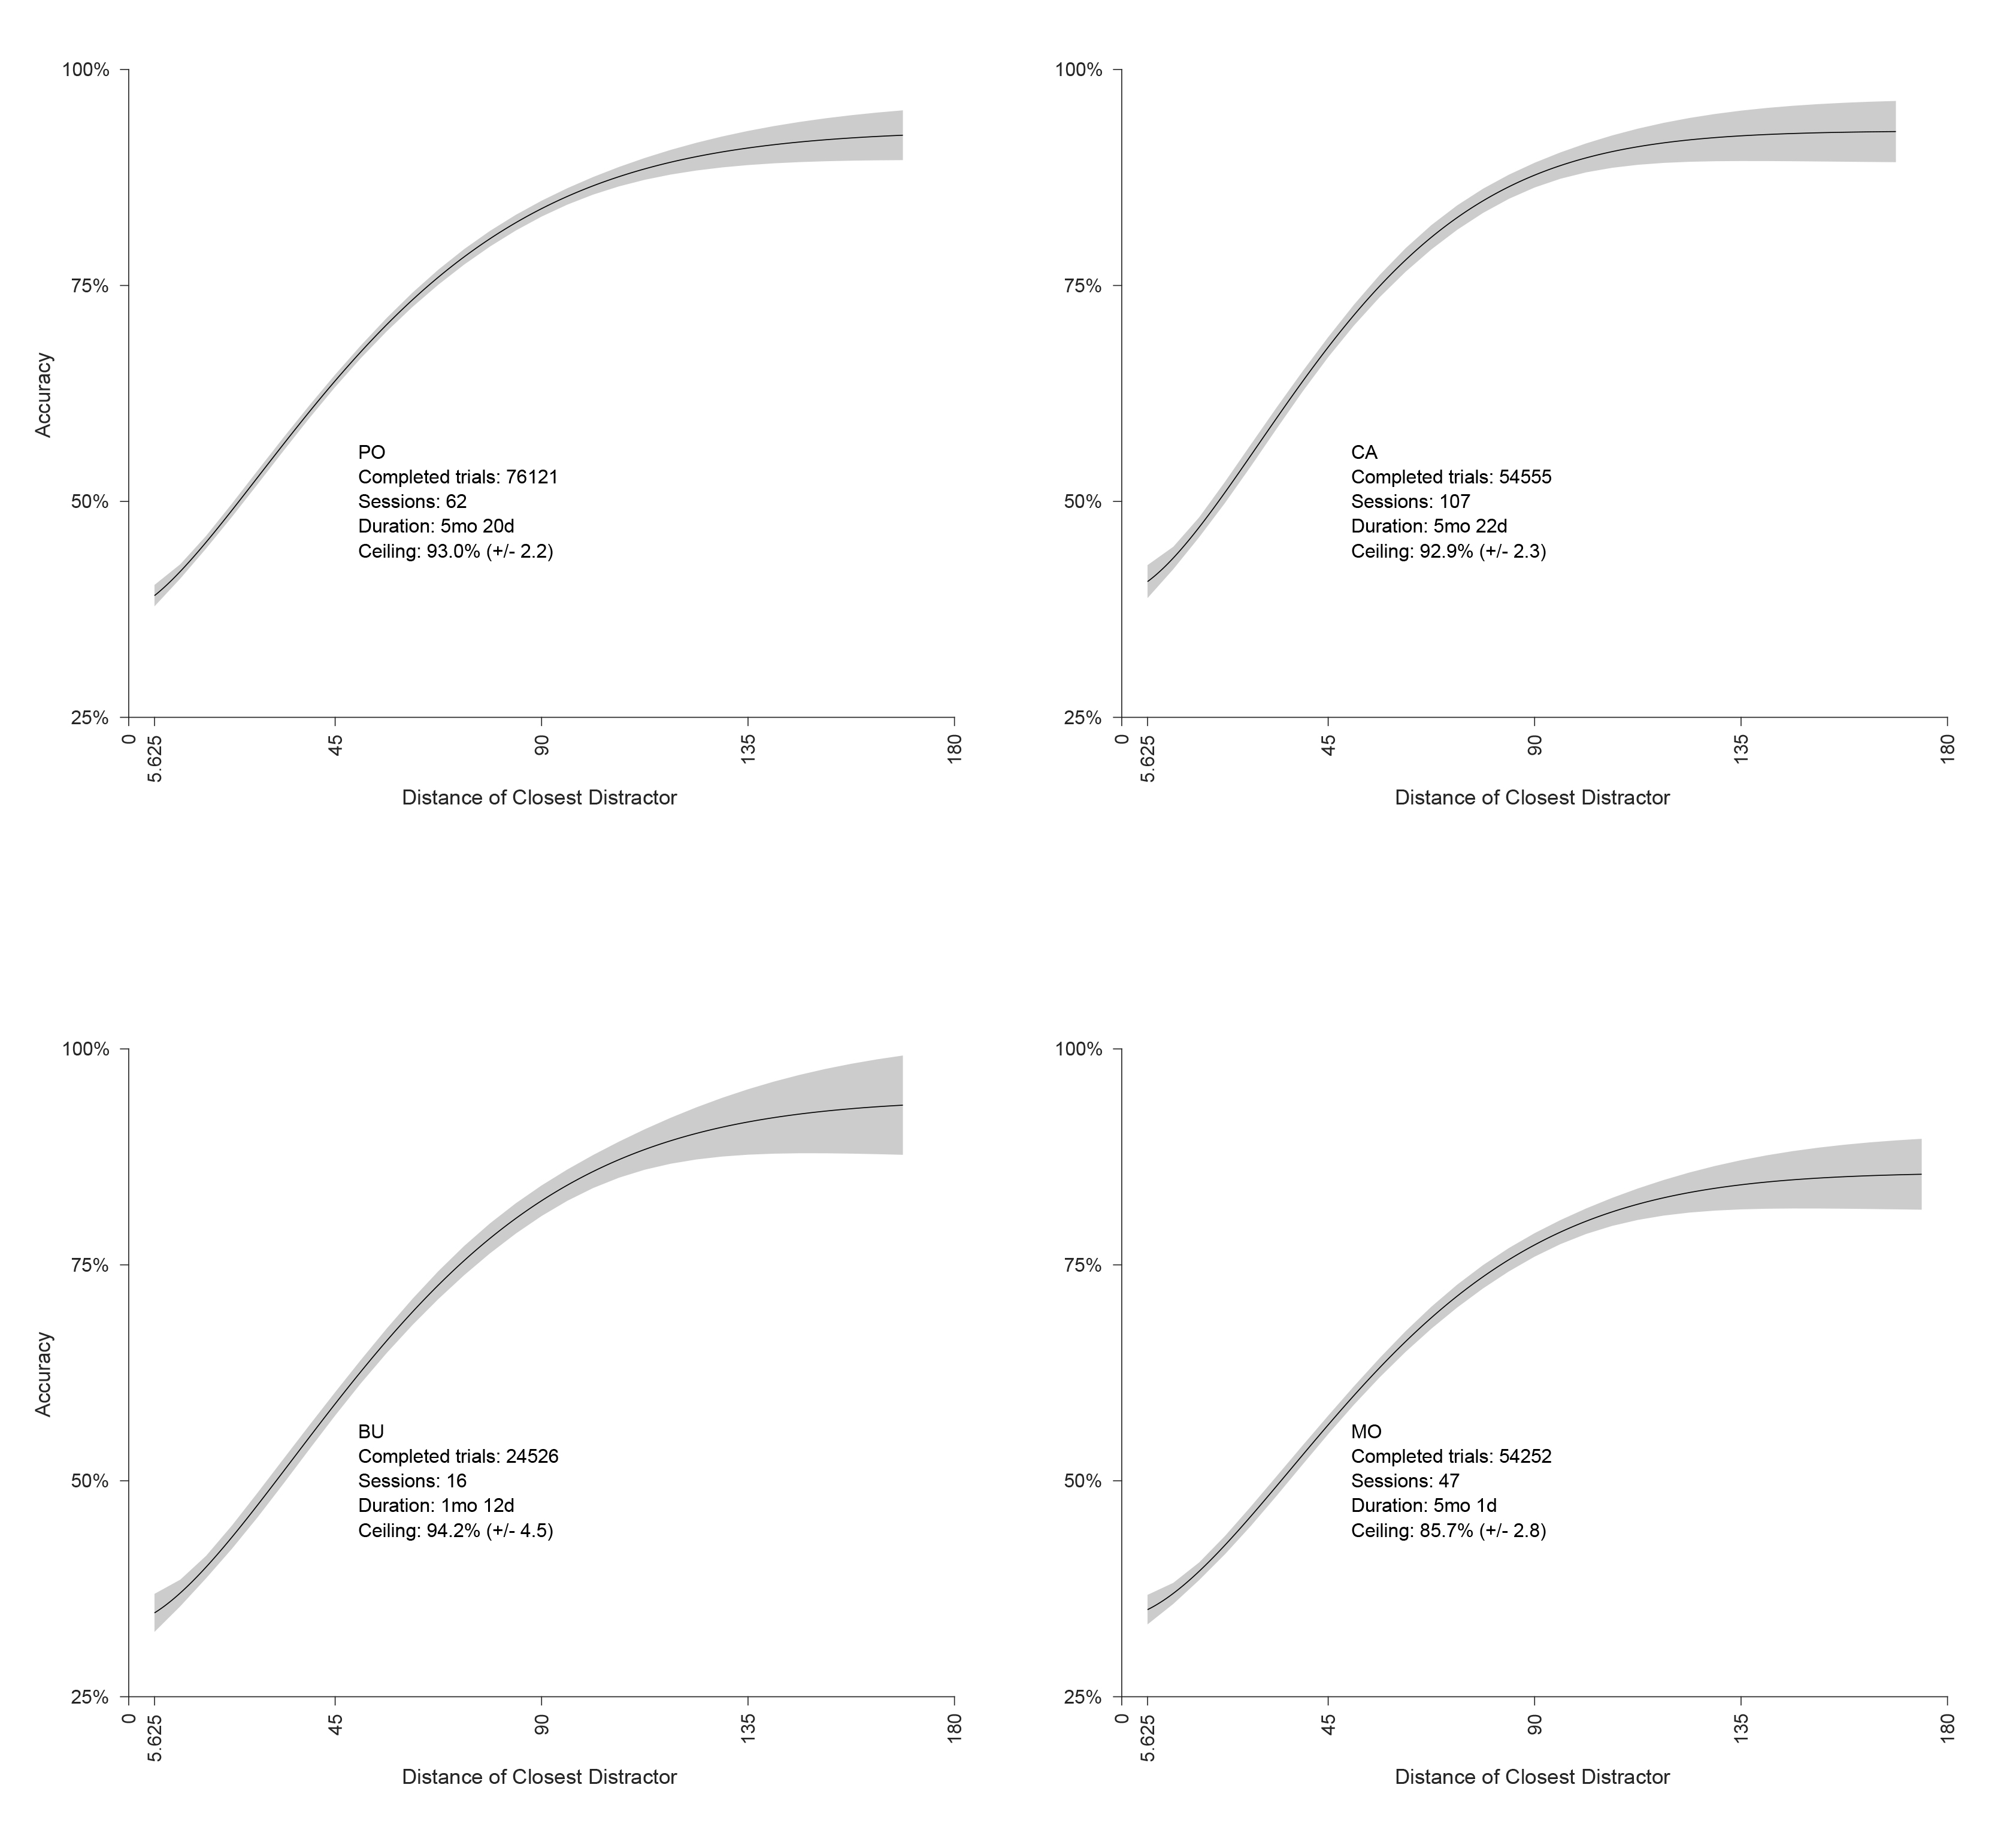
\includegraphics[width=\textwidth+4cm]{../Figures/flat/SI1_psychometric.jpg}
    \caption{\textbf{Psychometric functions for the four individual animals (PO, CA, BU, MO) on the color-matching task illustrated in Figure 1.}
    Completed trials for the four animals were: 76121; 54555; 24526; 54252.
    } 
    \label{fig:IndiDiff}
    \end{fullwidth}
\end{figure}

\begin{figure}
    \centering
    \begin{fullwidth}
    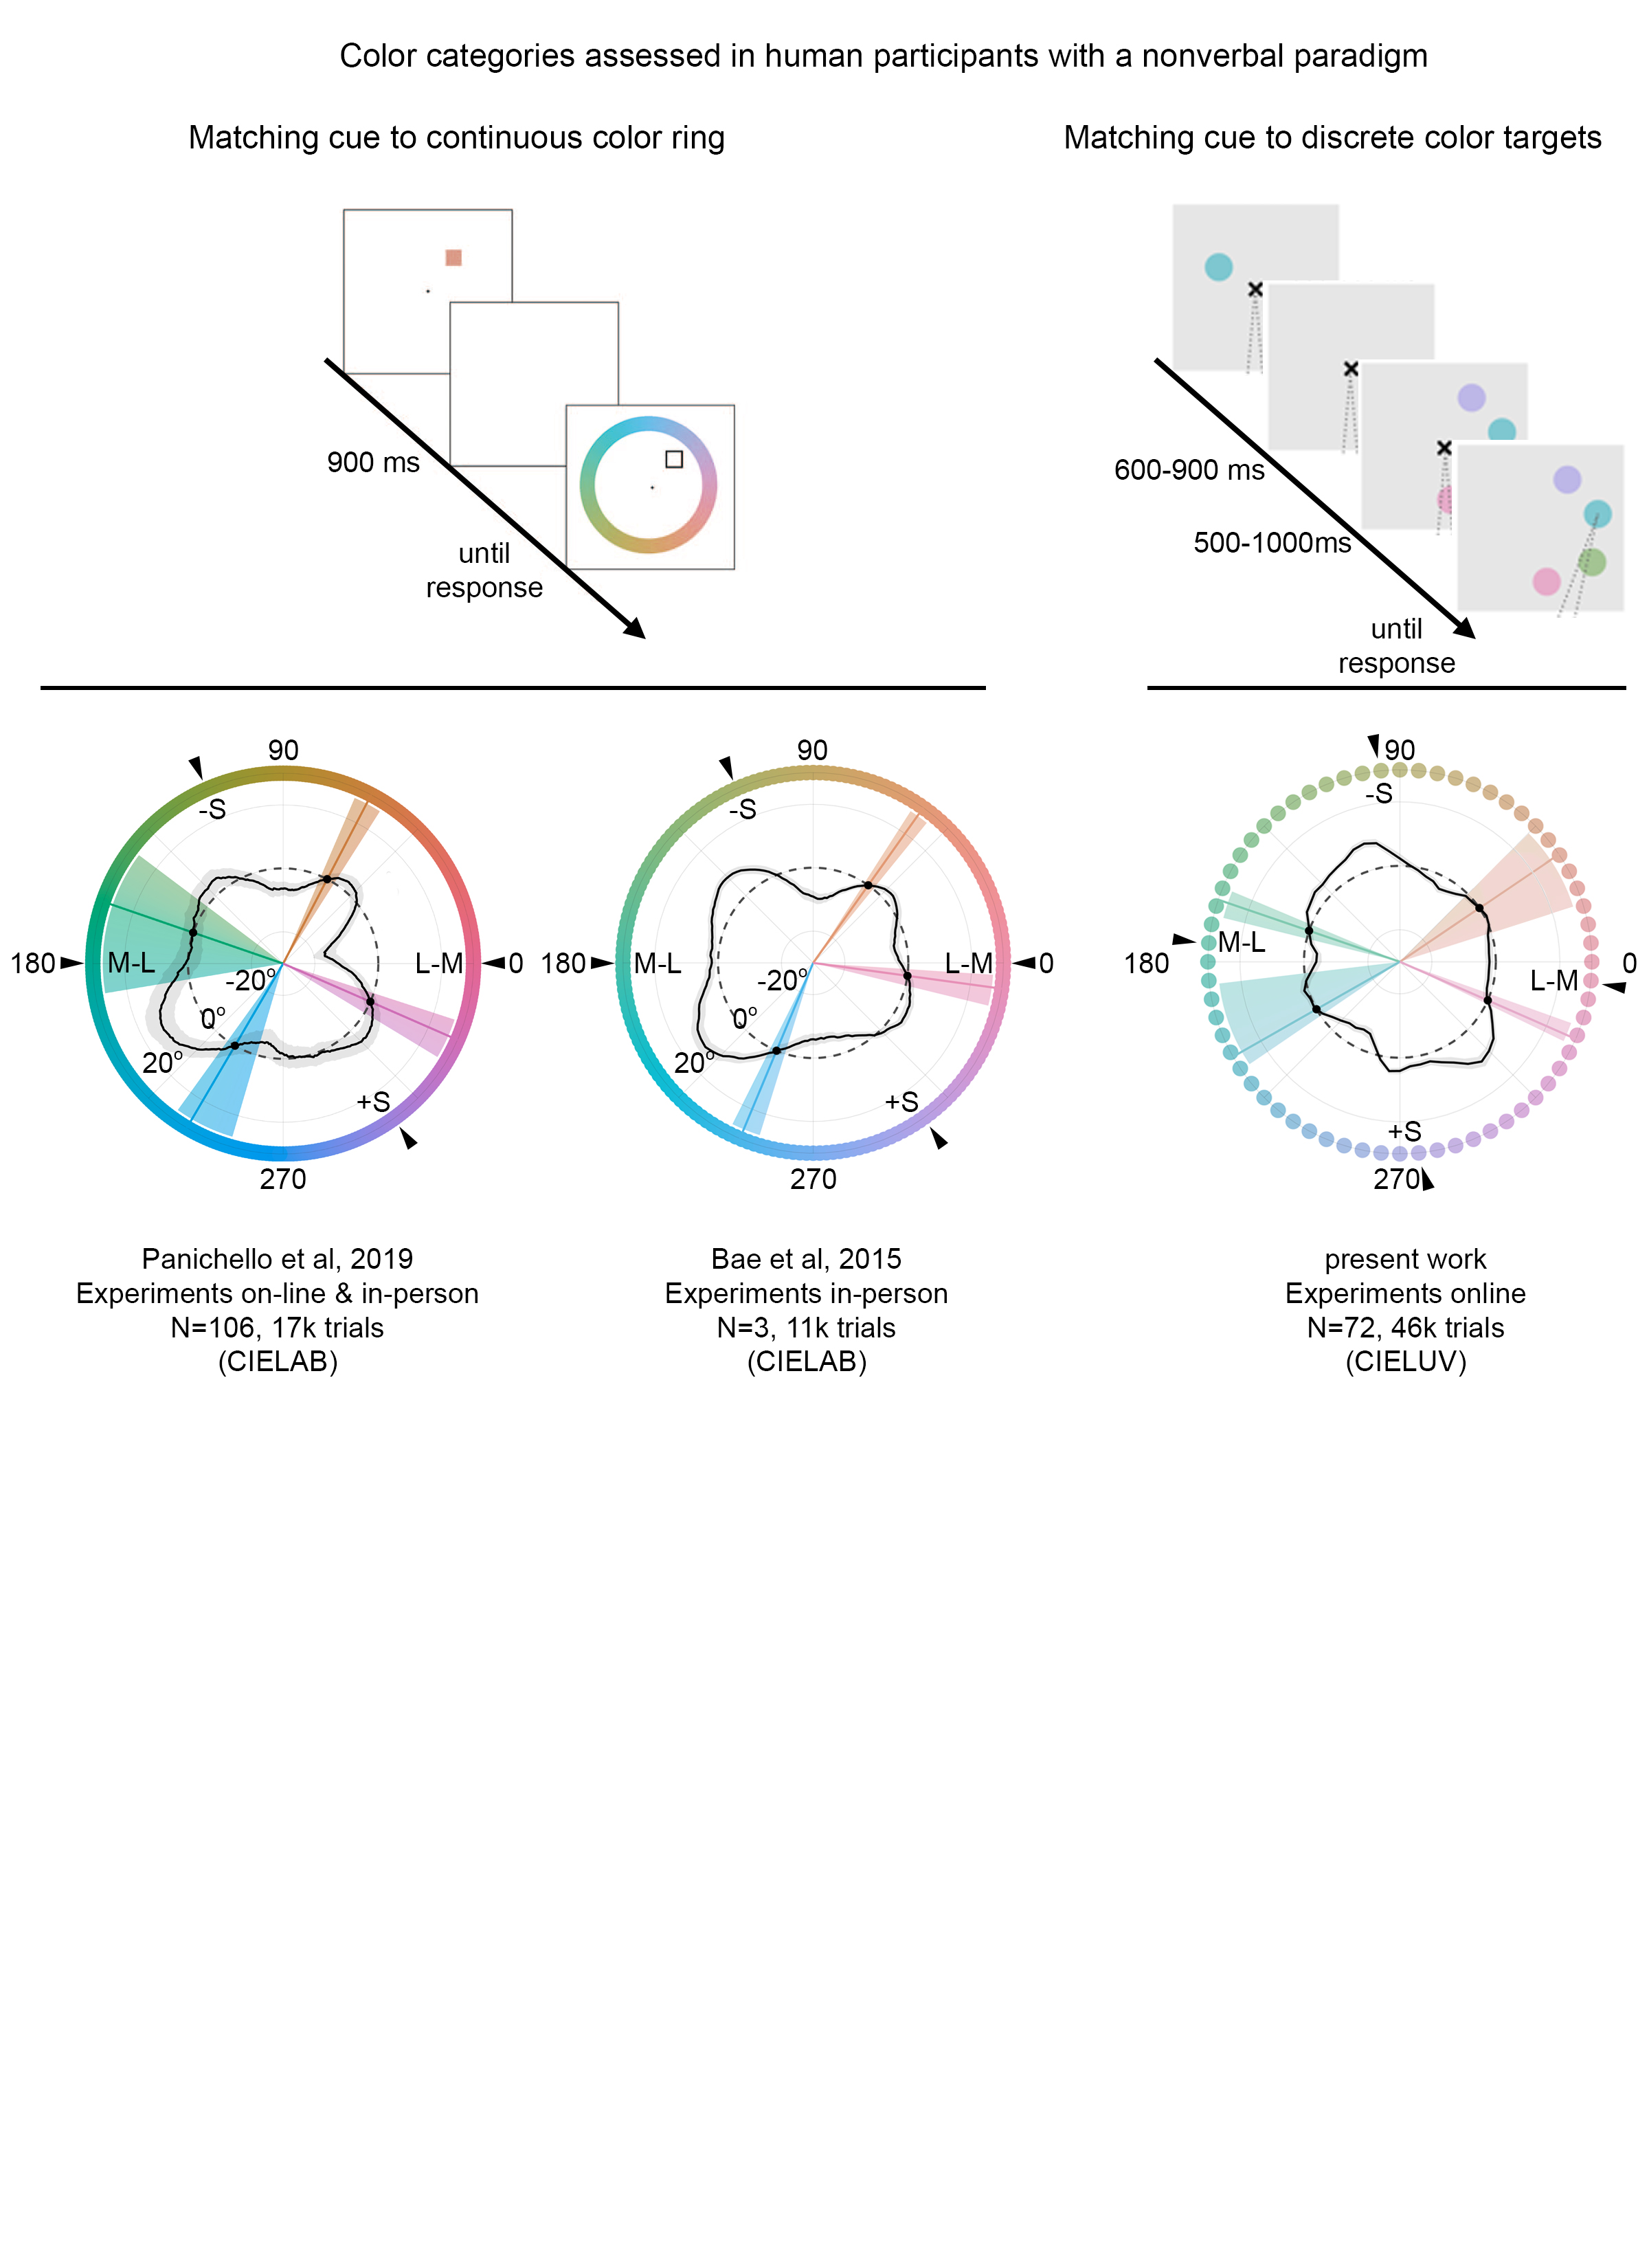
\includegraphics[width=\textwidth+4cm,trim={0 11cm 0 0},clip]{../Figures/flat/SI_Human_2.jpg}
    \caption{\textbf{Color categories assessed in human participants with a nonverbal paradigm. }
    Prior work by \citet{bae_why_2015} and \citet{panichello_error-correcting_2019} has used a task in which participants match the color of a cue to a continuous ring of colors; those published results were obtained with a combination of in-person experiments and on-line experiment, with a memory delay and without. The results are broadly consistent, recovering four color categories by mixture-model analysis, corresponding to blue, green, orange and pink. 
    Note that the data from \citep{bae_why_2015} shown in the figure were from just three participants, engaged in a task that had a memory delay; those authors confirmed the results in more subjects with a version of the task that omitted the memory delay period (the cue and the match-option color wheel were presented simultaneously). The present work adapted the paradigm so that the match options in each trial were four discrete targets randomly drawn from 64 colors sampling the color space. The data shown in this figure were obtained in human participants, with experiments conducted online with Amazon Mechanical Turk. These results are again broadly consistent with the prior work using the continous-matching ring in recovering, by mixture analysis, four significant categories corresponding to blue, green, orange, and pink. We note that the discrete-matching task recovers a trend for a fifth category that would correspond to “purple”; close inspection of the results in \citep{bae_why_2015, panichello_error-correcting_2019} and in studies of human infants \citep{skelton_biological_2017} also show evidence of this trend. The stimuli in the \citep{bae_why_2015, panichello_error-correcting_2019} were defined in CIELAB, while the stimuli in the present work were defined in CIELUV; this difference in color space is associated with a slight clockwise rotation of the cone-opponent axes. The S axis poles provide a useful landmark; they are associated with negative slopes in all three data sets.
    } 
    \label{fig:Human}
    \end{fullwidth}
\end{figure}

\begin{figure}
    \centering
    \begin{fullwidth}
    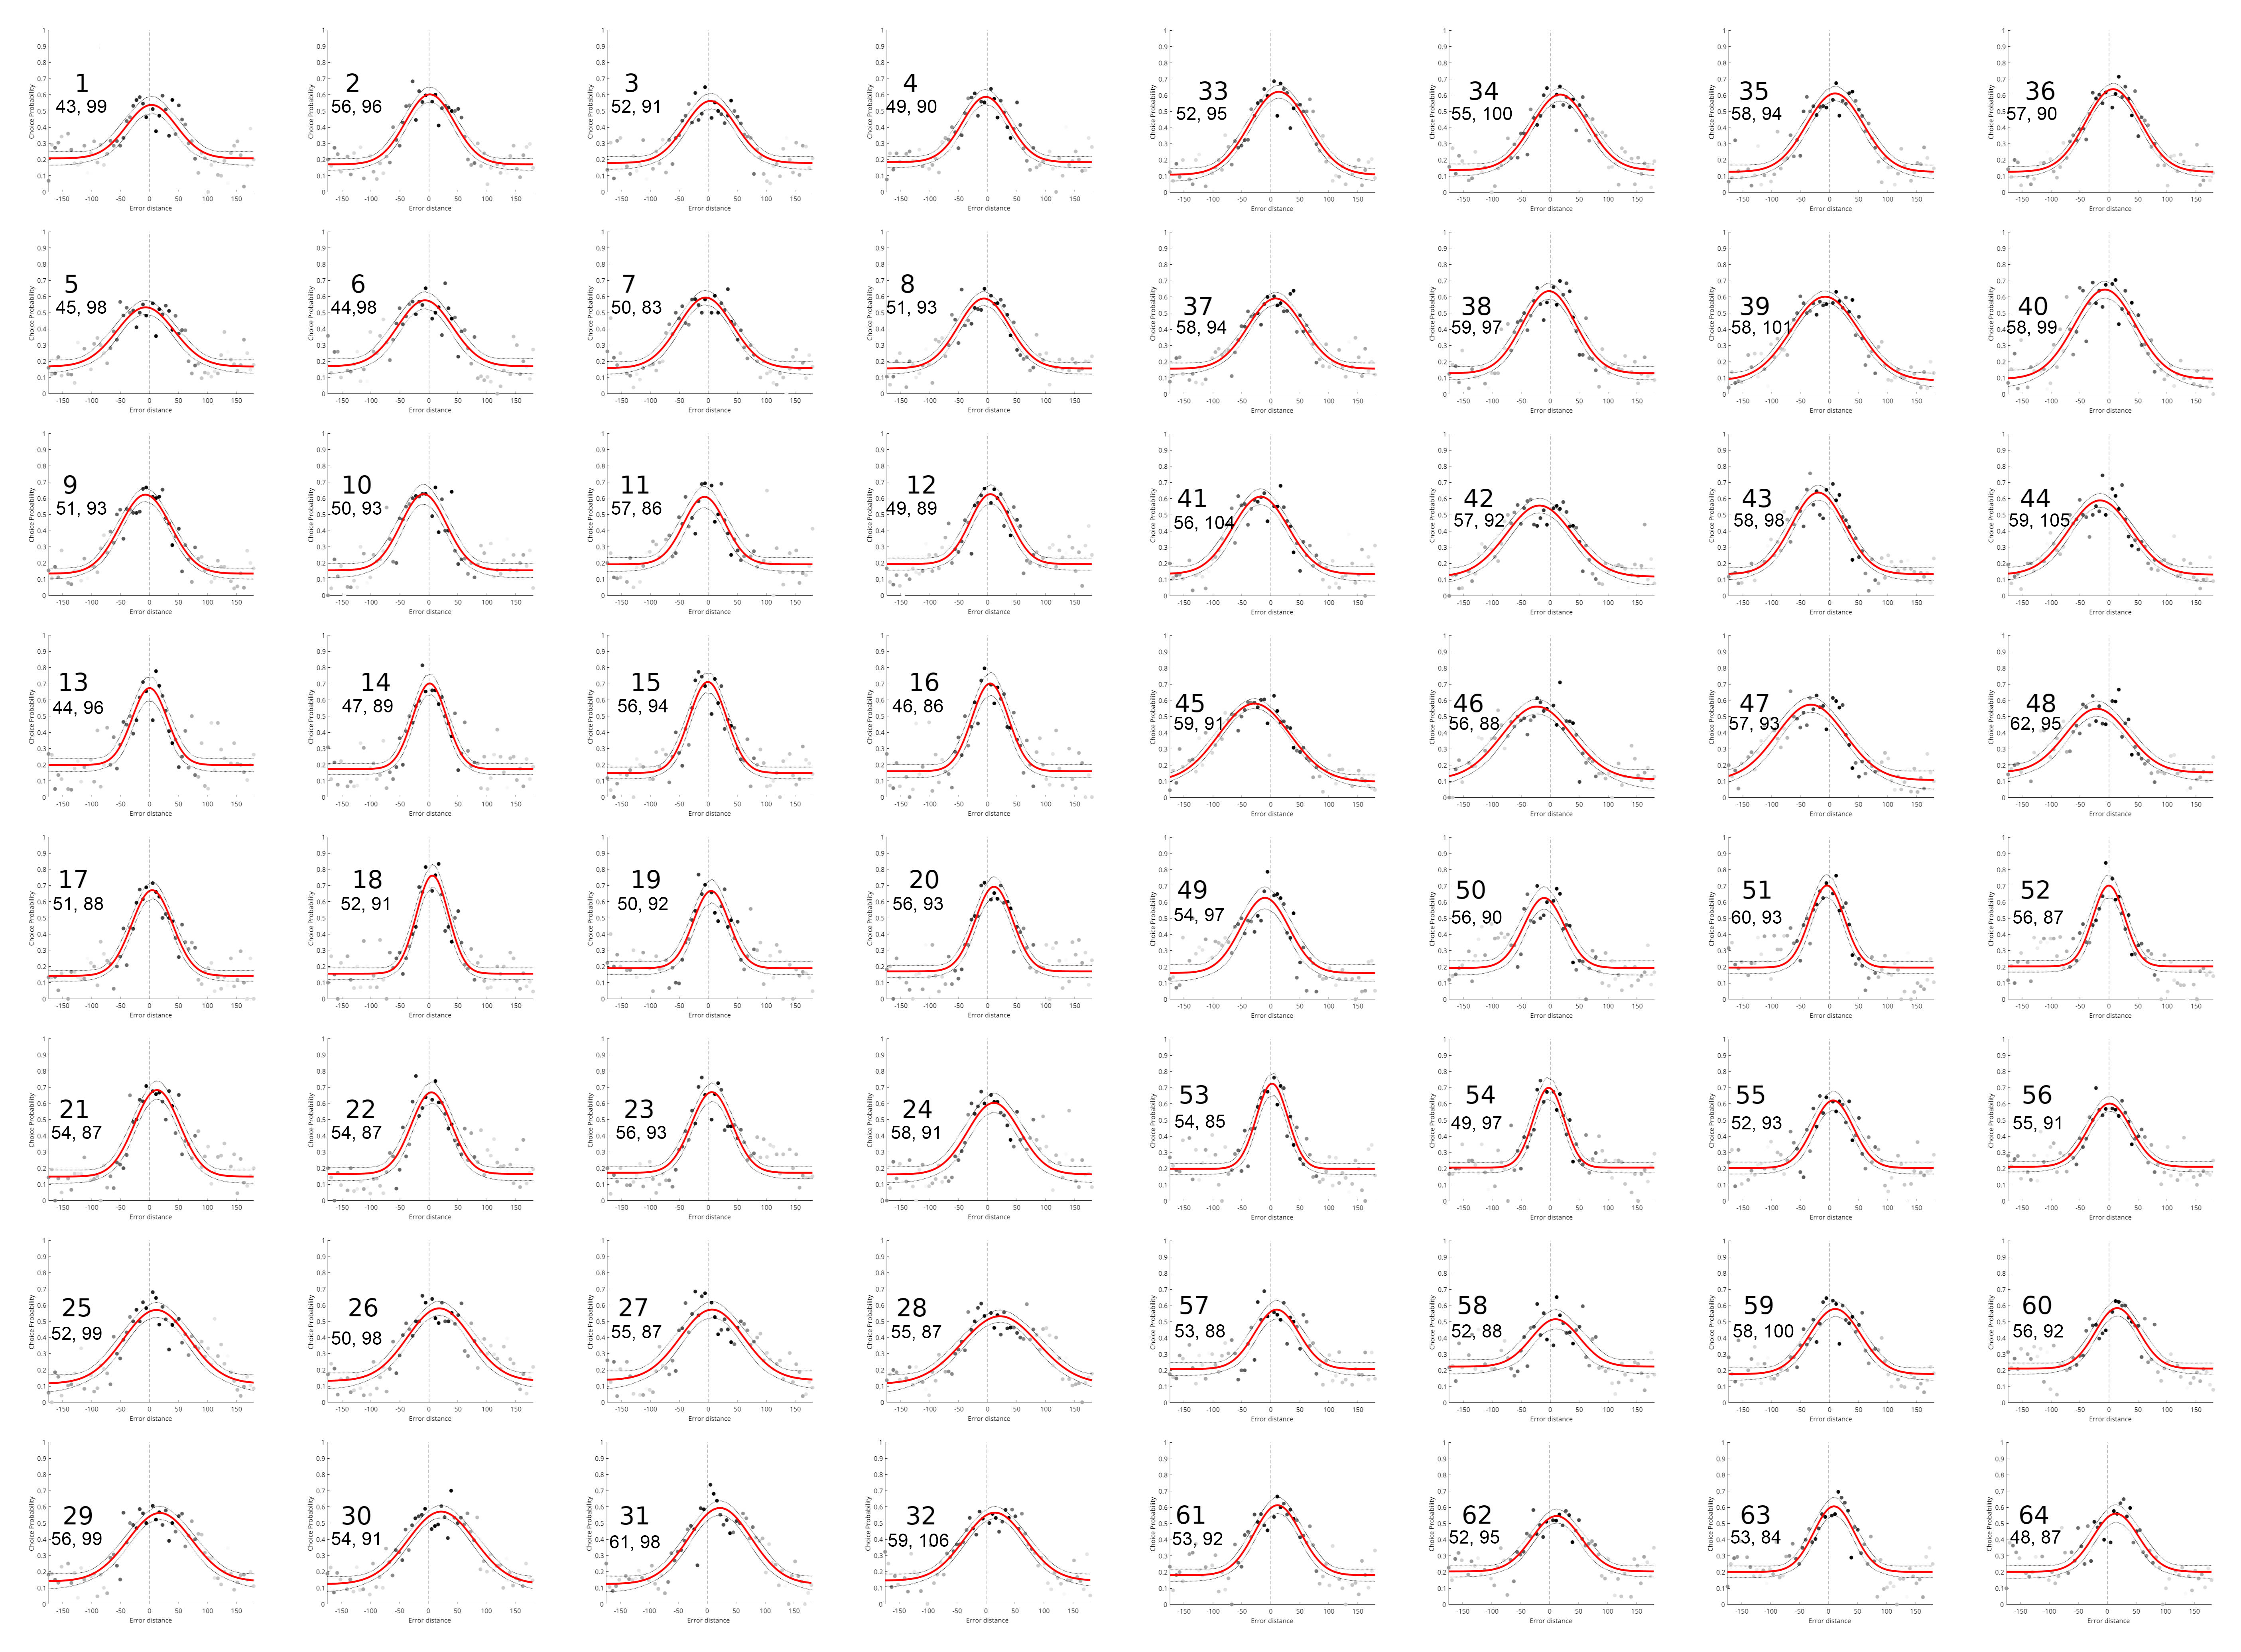
\includegraphics[width=\textwidth+4cm]{../Figures/flat/SI3_MMBreakOut_2.jpg}
    \caption{\textbf{Gaussian fits from the Mixture Model.}
    Each trace shows the Gaussian fit for one of the 64 target colors (large number in each panel corresponds to the cue color) used in the color-matching task, as per Equation 1; data averaged over four animals. The extent to which each data point is black versus white indicates the number of trials that provided that choice option, normalized for each cue (the pair of smaller numbers below the cue-color number provides the range: the larger number corresponds to the black symbol, and the smaller number to white); see Methods for how the curves were fit to the data. 
    } 
    \label{fig:MMBreakOut}
    \end{fullwidth}
\end{figure}

\begin{figure}
    \centering
    \begin{fullwidth}
    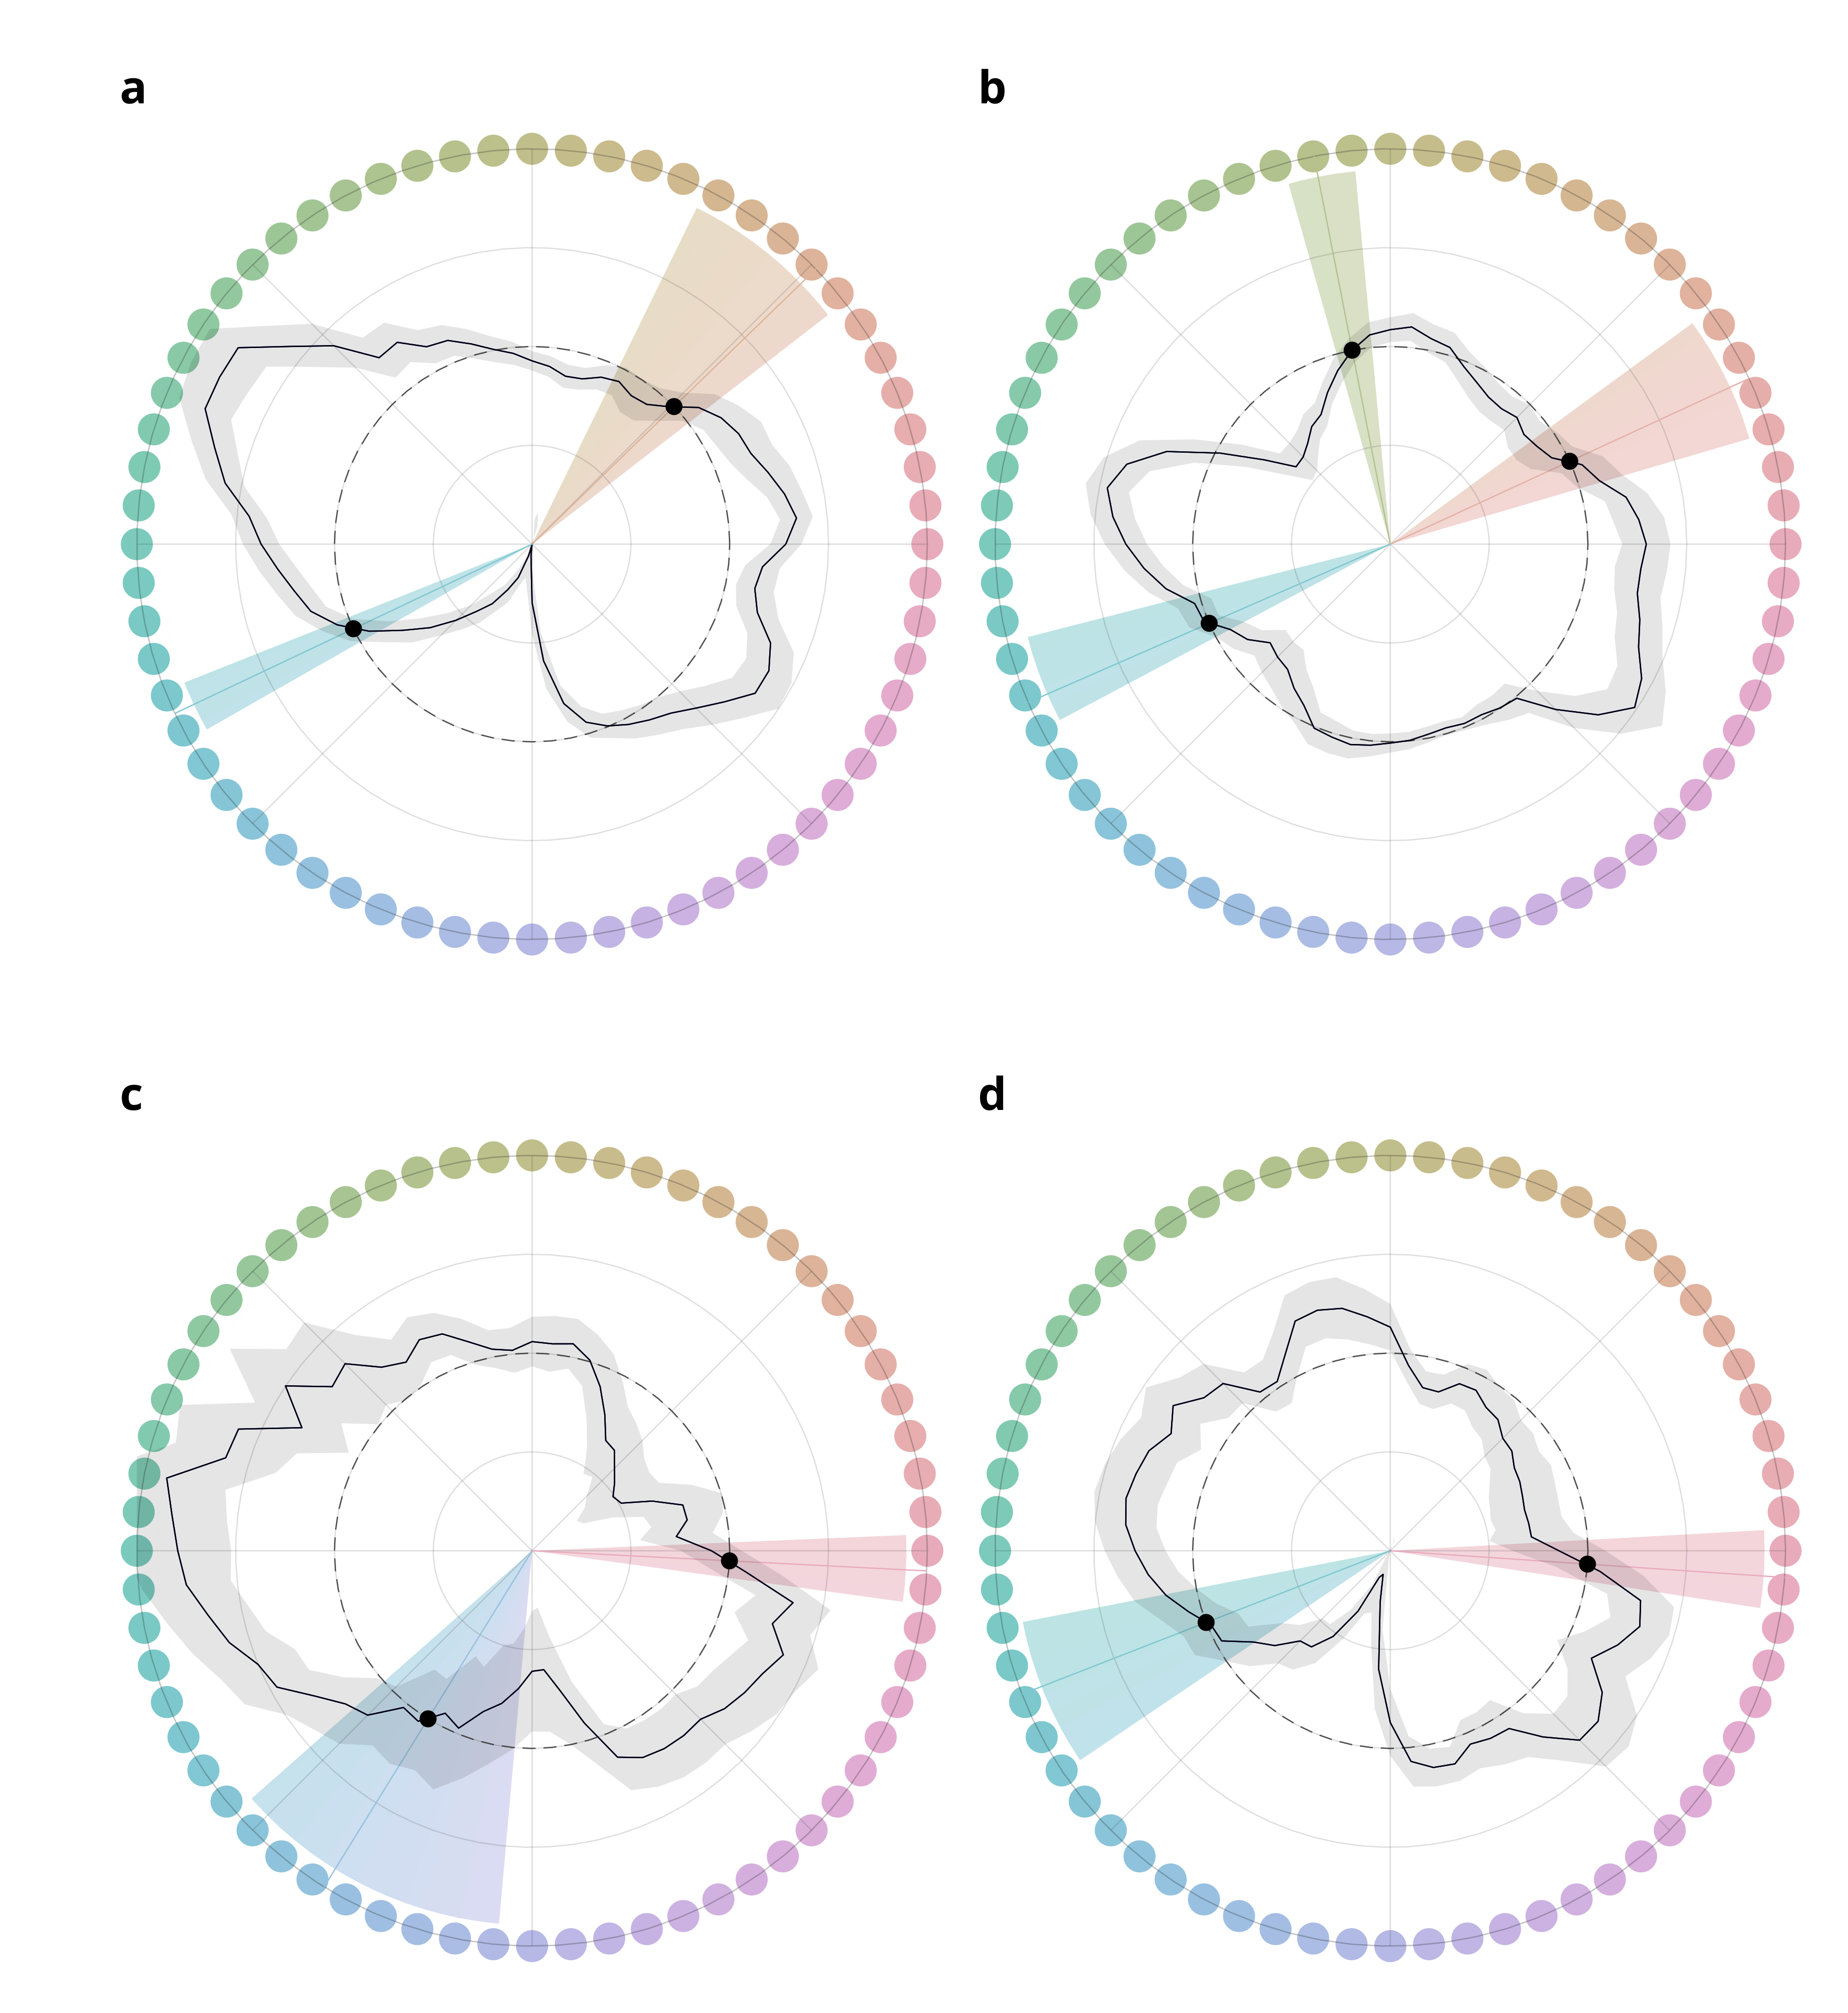
\includegraphics[width=\textwidth+4cm]{../Figures/flat/SI4_MM.jpg}
    \caption{\textbf{Mixture-model analysis of the individual data for the four animals in the color-matching task.}
    Data shown in the same format as Figure 2c; data subsampled to ensure the same amount of data per animal (24526 trials; note that this included all the completed trials for the monkey whose data are shown in panel c).
    } 
    \label{fig:IndiMM}
    \end{fullwidth}
\end{figure}

\begin{figure}
    \centering
    \begin{fullwidth}
    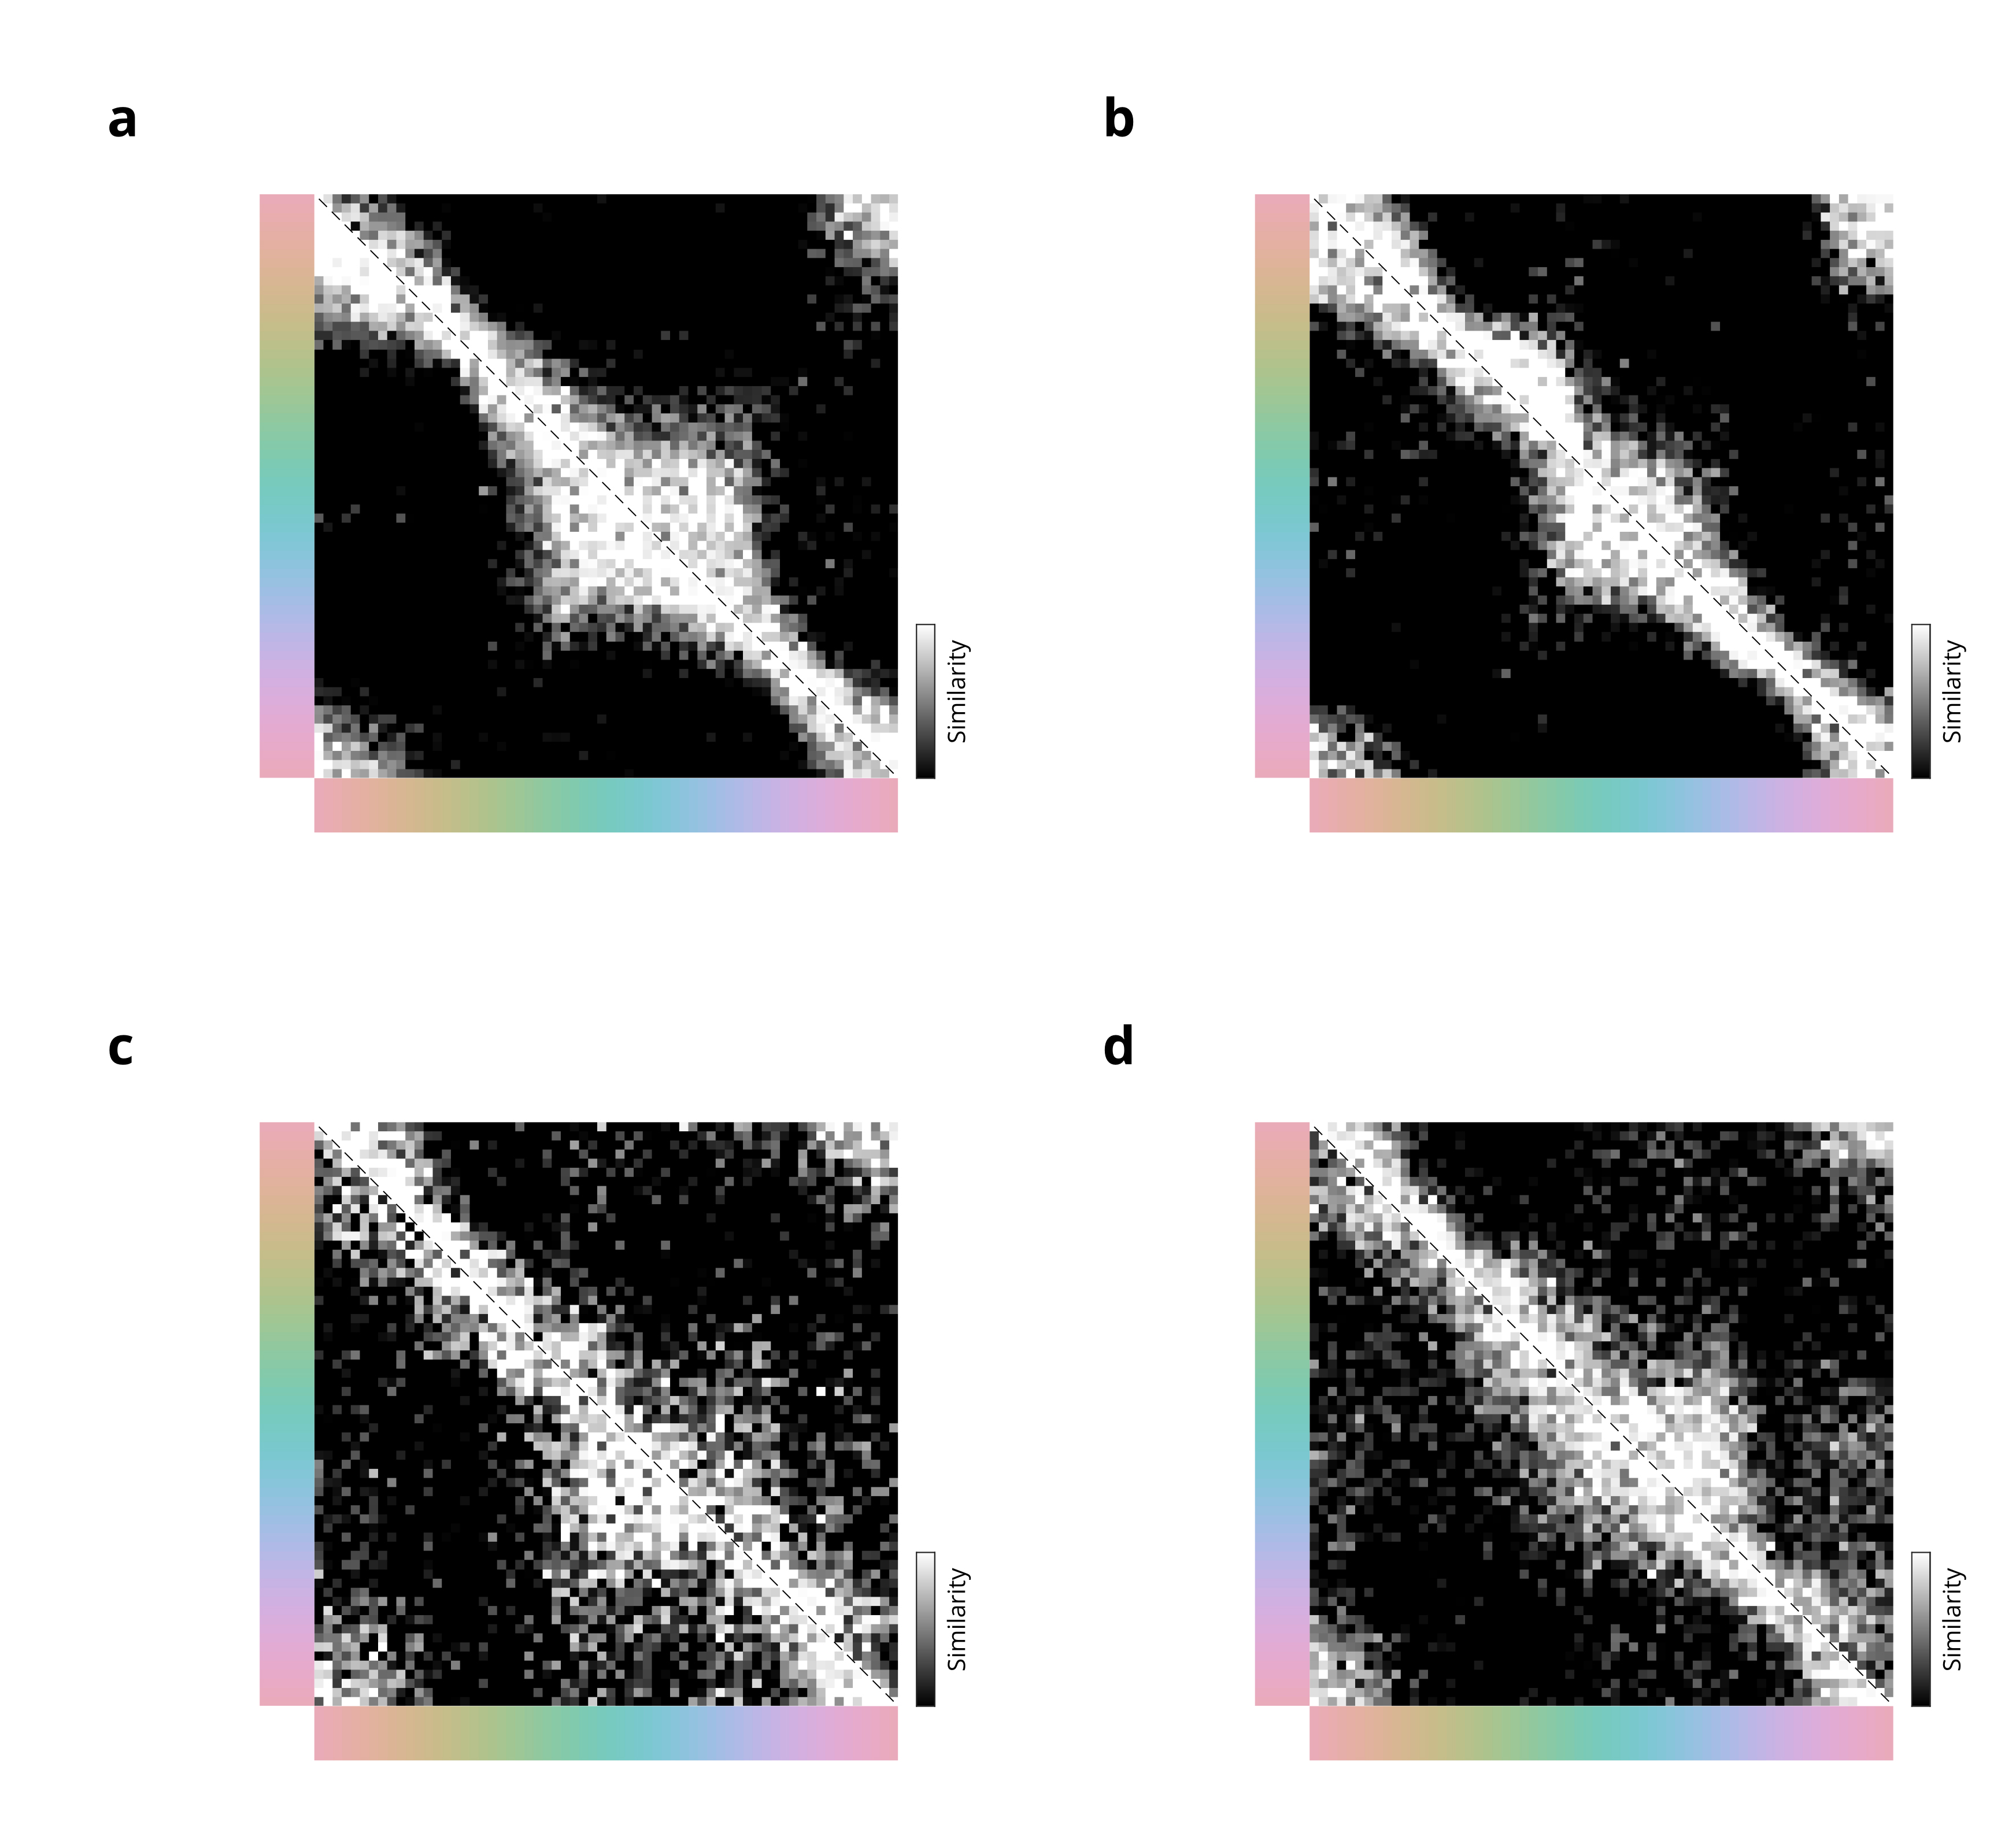
\includegraphics[width=\textwidth+4cm]{../Figures/flat/SI5_IndTCCv.jpg}
    \caption{\textbf{Similarity matrices for free similarity matrix models, fit to individual data.}
    The order of the plots is the same as the order in other figures, PO, CA, BU, MO. See Figure 3ab for data averaged across animals, with data subsamples to ensure the same amount of data per animal.
    } 
    \label{fig:IndiTCC}
    \end{fullwidth}
\end{figure}

\begin{figure}
    \centering
    \begin{fullwidth}
    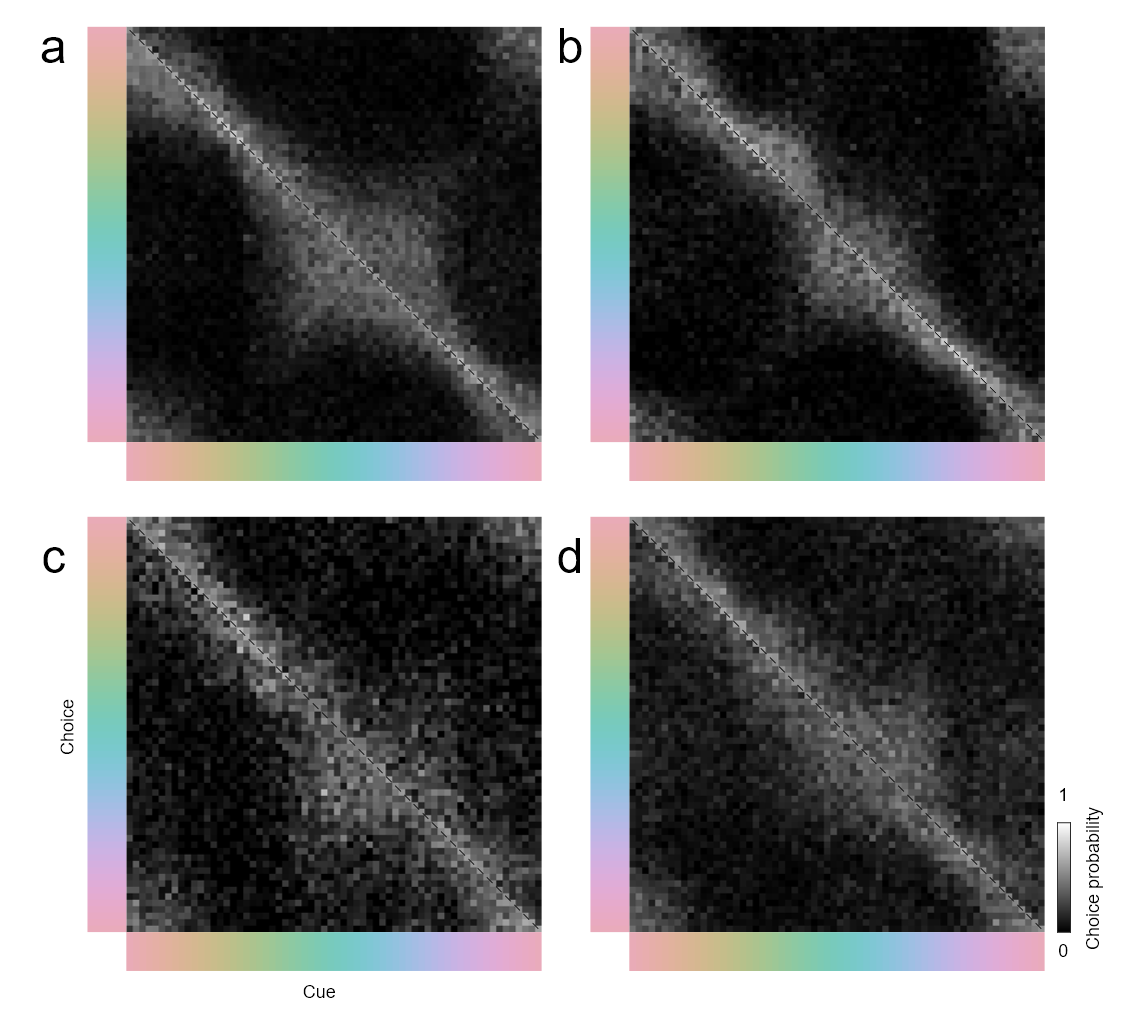
\includegraphics[width=\textwidth+4cm]{../Figures/flat/SI6_choiceMatrices.png}
    \caption{\textbf{Choice probability matrices for free similarity matrix models, for the four individuals.}
    As per the similarity matrices presented, each column represents a cue, and each row represents a choice. 
    Here, however, rather than the similarity between cue/choice pairs we show the probability of selection. 
    Whereas the similarity matrix is the output of model fitting, this matrix is derived more directly from the data: each cell is simply the number of times a particular choice was made divided by the number of times that choice was an option. 
    The identity line, representing correct options, appears artifically inflated (see Methods for further information).
    } 
    \label{fig:choiceProbabilityMatrices}
    \end{fullwidth}
\end{figure}






%%%%%%%%%%%%%%%%%%%%%%%%%%%%%%%%%%%%%%%%%%%%%%%%%%%%%%%%%%%%
%%% ARTICLE END
%%%%%%%%%%%%%%%%%%%%%%%%%%%%%%%%%%%%%%%%%%%%%%%%%%%%%%%%%%%%

\end{document}




